\documentclass[12pt,nopreprintline]{elsarticle}
\usepackage[utf8]{inputenc}
\usepackage[T1]{fontenc}
\usepackage[top=2.4cm,bottom=2.2cm,left=2.0cm,right=2.0cm]{geometry}
\usepackage[english]{babel}
\usepackage[table,dvipsnames]{xcolor}
\usepackage{graphicx,array,booktabs,longtable,multirow,tabularx}
\usepackage{amsmath,amssymb,amsthm,mathrsfs,bm}
\usepackage{float,placeins,caption,setspace,gensymb,wasysym,times}
\usepackage{needspace}
\usepackage{tikz,tikz-qtree}
\usetikzlibrary{arrows,arrows.meta,automata,positioning,calc,decorations.pathreplacing,decorations.pathmorphing,trees,shapes.misc}
\usepackage{etoolbox}
\usepackage[colorlinks=true,allcolors=black]{hyperref}
\urlstyle{same}
\AtBeginDocument{\hypersetup{allcolors=black}}
\definecolor{RevisionBlue}{RGB}{23,64,156}
\definecolor{RevisionRed}{RGB}{169,25,35}
\definecolor{nGray}{RGB}{214,214,214}
\definecolor{intnull2}{RGB}{214,214,214}
\newenvironment{revision}{\begingroup\color{RevisionBlue}\hypersetup{allcolors=RevisionBlue}}{\par\endgroup}
\DeclareRobustCommand{\rev}[1]{{\color{RevisionBlue}\hypersetup{allcolors=RevisionBlue}#1}}
\newenvironment{redrevision}{\begingroup\color{RevisionRed}\hypersetup{allcolors=RevisionRed}}{\par\endgroup}
\DeclareRobustCommand{\revred}[1]{{\color{RevisionRed}\hypersetup{allcolors=RevisionRed}#1}}
\pdfstringdefDisableCommands{\def\rev#1{#1}\def\revred#1{#1}}
\AtBeginEnvironment{thebibliography}{%
  \let\savedbibitem\bibitem
  \renewcommand{\bibitem}[2][]{%
    \color{black}\hypersetup{allcolors=black}%
    \ifboolexpr{test {\ifstrequal{#2}{zhang2025myoelectric}} or test {\ifstrequal{#2}{zhang2024fall}} or test {\ifstrequal{#2}{chen2022computer}} or test {\ifstrequal{#2}{sethi2022comprehensive}} or test {\ifstrequal{#2}{scataglini2024accuracy}} or test {\ifstrequal{#2}{boswell2021neural}}}{\color{RevisionBlue}\hypersetup{allcolors=RevisionBlue}}{}%
    \ifboolexpr{test {\ifstrequal{#2}{wade2023examination}} or test {\ifstrequal{#2}{uhlrich2023opencap}} or test {\ifstrequal{#2}{augustine2025clothing}} or test {\ifstrequal{#2}{viswakumar2022omgait}} or test {\ifstrequal{#2}{lee2023lowlight}} or test {\ifstrequal{#2}{wu2012illumination}}}{\color{RevisionRed}\hypersetup{allcolors=RevisionRed}}{}%
    \savedbibitem[#1]{#2}}}
\newcommand{\etal}{\textit{et al}}
\newcommand{\etc}{\textit{etc.}}
\newcommand{\citeColored}[2]{\cite{#2}}
\setstretch{1}
\setlength{\emergencystretch}{2em}
\captionsetup[table]{position=top,skip=7pt}
\setlength{\LTpre}{7pt}
\setlength{\LTpost}{7pt}
\setlength{\LTcapwidth}{\textwidth}
\journal{Neural Networks}

\begin{document}
\begin{frontmatter}

\title{\textbf{Vision-Based Gait Analysis for Identifying Lower-Limb Joint Mobility Disorders: A Comprehensive Survey}}

\author[bitsc]{Vikas Kumawat}
\ead{p20210020@pilani.bits-pilani.ac.in}
\author[BU]{Hari Mohan Pandey}
\ead{hpandey@bournemouth.ac.uk, profharimohanpandey@gmail.com}
\author[bitsc]{Yashvardhan Sharma}
\ead{yash@pilani.bits-pilani.ac.in}
\author[bitsc]{Ashutosh Bhatia}
\ead{ashutosh.bhatia@pilani.bits-pilani.ac.in}
\author[jain]{Kamlesh Tiwari}
\ead{kamlesh.tiwari@jainuniversity.ac.in}

\address[bitsc]{Department of CSIS, Birla Institute of Technology and Science Pilani, Rajasthan, INDIA, 333031}
\address[BU]{School of Computing and Engineering, Bournemouth University, United Kingdom} 
\address[jain]{Department of CSE, Jain University, Bangalore, INDIA}

\begin{abstract}
\begin{revision}
Lower-limb joint mobility problems (JMPs) affect walking through changes in joint motion, loading and compensation. Video offers a practical way to measure some of these changes, but its value depends on the variable, the recording conditions and the population studied. This survey brings together clinical gait studies and computer-vision research on the hip, knee and ankle. It first identifies the gait variables associated with impairment at each joint, then examines how action recognition, gait analysis and pose estimation can recover or interpret those variables. The survey extends earlier reviews of clinical gait, rehabilitation and pose estimation by linking each candidate measurement to its reference standard and the evidence needed for interpretation. The literature supports video-based estimation of selected spatiotemporal and kinematic measures under the conditions studied. Estimates of joint loading, disease severity and future falls require different forms of validation. Small or unrepresentative cohorts, varied evaluation protocols and sensitivity to recording conditions limit the transfer of results to routine care. \revred{The survey helps identify measures to evaluate for repeat video assessment and where a more detailed biomechanical reference is needed.}
\end{revision}

\end{abstract}

\begin{keyword}
Human Action Recognition\sep Human Pose Estimation \sep Gait Analysis \sep Joint Mobility \sep Neural Network \sep Computer Vision \sep \rev{Markerless motion capture \sep Clinical validation.} 
\end{keyword}

\end{frontmatter}

\section{Introduction}
\label{sec:introduction}
\begin{revision}
Hip, knee and ankle disorders can change how a person walks well beyond the affected joint. Pain, restricted motion and weakness may alter walking speed, stride length, joint angles and loading, while compensatory movements emerge at the pelvis, trunk or neighbouring joints \cite{hertling2006management,ornetti2010gait,astephen2008biomechanical,shakoor2003asymmetric,ro2019effects}. Gait analysis therefore provides information about functional impairment and recovery. The difficulty is deciding which changes a measurement system can capture reliably and what they mean for a particular patient.

Clinical gait laboratories combine motion capture with force measurements and biomechanical models. These systems provide detailed measurements, but repeated assessment requires equipment, space and specialist support \cite{hulleck2022present,prakash2018recent}. Markerless methods estimate body landmarks and gait variables from RGB or depth video and have been evaluated for gait measurement and rehabilitation \cite{stenum2021two,uccheddu2022rgb,wang2024markerless,stenum2024clinical}. Agreement with a reference system depends on which variable is measured. A system that measures step time well still needs separate validation for ankle rotation \cite{scataglini2024accuracy}.

$-$\noindent\textbf{Positioning of the review.} Walking speed can reveal a change in mobility, but understanding which joint is affected requires more specific measures. Earlier reviews describe clinical gait assessment, rehabilitation methods and the performance of capture systems. This review builds on that work by linking the variables relevant to the hip, knee and ankle to video outputs and the evidence needed to interpret them. Section~\ref{sec:review_positioning} explains this relationship in more detail.

$-$\noindent\textbf{Scope and contribution.} This survey considers which gait findings associated with hip, knee and ankle joint mobility problems (JMPs) can be assessed from video and what evidence is needed to interpret those measurements. It makes three contributions.
\begin{itemize}
\item It draws on clinical studies to identify relevant gait variables for each joint, accounting for compensatory movement elsewhere in the lower limb.
\item It relates candidate measures to the vision methods and reference measurements used to estimate them. Action-recognition studies inform the choice of movement representation, while clinical studies establish which outputs have been validated in the intended population.
\item It sets out the evidence required for movement measurement, gait-pattern recognition and clinical inference, including severity assessment and prediction of future risk. Sections~\ref{sec:JMPWTCV} and~\ref{sec:KO} show how these requirements apply to specific joints and outcomes.
\end{itemize}

Fall-related gait research illustrates the difference between recognising a movement pattern and estimating a clinical outcome. Chen et al. \cite{chen2022computer} use camera-derived kinematics. Two studies by Zhang et al. \cite{zhang2025myoelectric,zhang2024fall} use surface electromyography (sEMG) to capture muscle activity. Section~\ref{sec:fall_related} compares the endpoints and explains what each study contributes to the assessment of joint mobility.
\end{revision}

\begin{redrevision}
$-$\noindent\phantomsection\label{loc:significance}\textbf{Significance of the study.}
For clinicians and rehabilitation teams, the practical question is which changes in walking can be followed from video between assessments. Timing a step and measuring ankle motion during swing, for instance, place different demands on camera position, landmark visibility and validation. By organising the evidence around the hip, knee and ankle, the survey helps readers choose measures that address the impairment of interest and recognise when a change may reflect compensation at another joint. It also helps developers choose the reference measurement, patient group and recording conditions needed to test a proposed method. These distinctions matter when deciding whether a video measure can support monitoring and when an instrumented assessment is needed.
\end{redrevision}

\begin{revision}
$-$\noindent\textbf{Paper organisation.} Figure~\ref{fig:timingdiagram} shows how the review is organised. Section~\ref{sec:methodology} describes the review method. Sections~\ref{sec:JMP} and~\ref{sec:JMPCV} give the clinical context, position the review and define the vision task. Sections~\ref{sec:JMPWTCV} and~\ref{sec:JMPWCV} examine the clinical and technical evidence. Sections~\ref{sec:discussion} and~\ref{sec:conclusion} discuss its implications for joint mobility assessment.
\end{revision}

\begin{figure} 
    \centering
    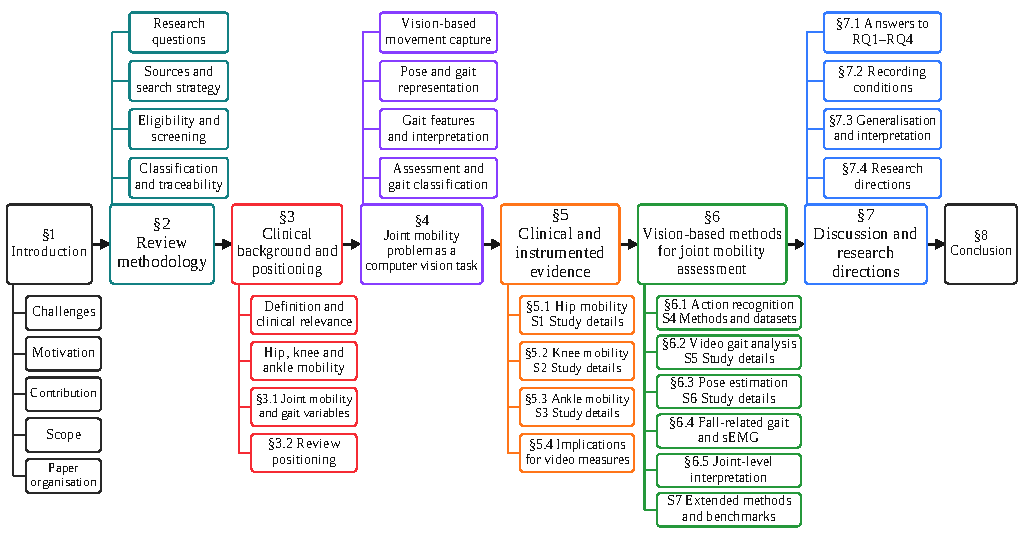
\includegraphics[width=\linewidth]{Images/Timing_Diagram.pdf}
    \caption{Time diagram that reflects the survey pipeline. The horizontal arrows show the order of Sections~1--8 in the main paper. Labels S1--S7 denote sections in the separate supplementary file.}
    \label{fig:timingdiagram}
\end{figure}

\FloatBarrier

\section{\revred{Review Methodology}}
\label{sec:methodology}
\begin{redrevision}
We used a structured narrative approach to bring together clinical gait studies and work on computer vision. The studies differ in the people they examine, the variables they report and the reference measurements they use. We therefore compare what individual findings support within their study conditions.
\end{redrevision}

\subsection{\revred{Review Design and Research Questions}}
\label{sec:review_questions}
\begin{redrevision}
The review starts with a clinical question about the hip, knee or ankle, identifies the gait variable that could help answer it, and examines how that variable is estimated and checked. Figure~\ref{fig:reviewaxes} illustrates these three dimensions with an ankle example. Table~\ref{tab:review_questions} sets out the research questions, and Section~\ref{sec:rq_discussion} discusses the evidence for each.
\end{redrevision}

\begin{figure} 
    \centering
    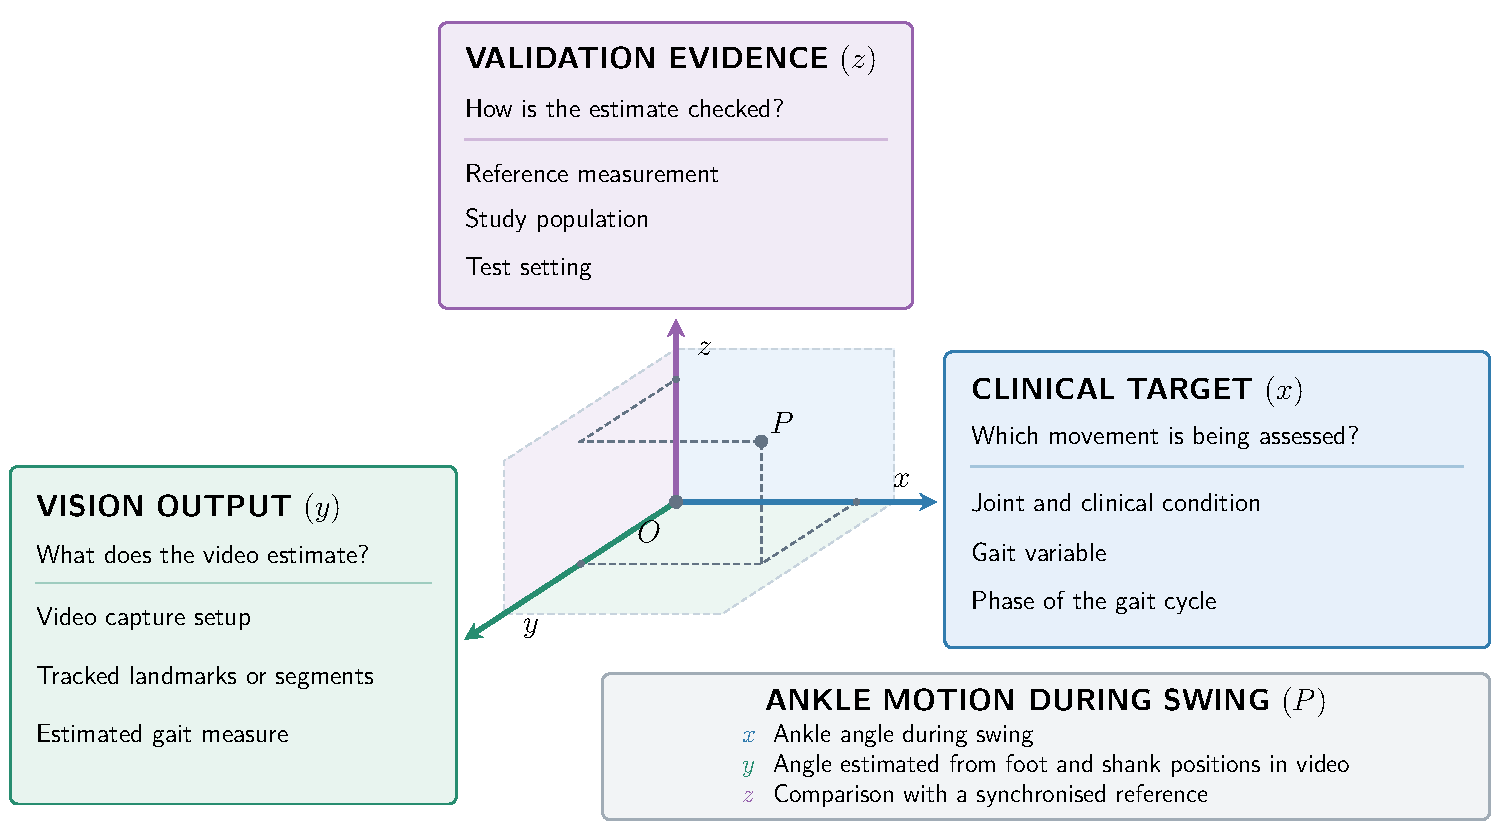
\includegraphics[width=0.75\linewidth]{Images/Figure_02_Gait_Review_Axes.pdf}
    \caption{Three qualitative dimensions of a joint mobility claim. The dashed guides project the ankle-swing example \(P\) onto the clinical target, vision output and validation evidence axes.}
    \label{fig:reviewaxes}
\end{figure}

%\input{Review_Dimensions}

\begin{table}[!htbp]
\centering\small
\caption{\revred{Research questions and where they are addressed.}}
\label{tab:review_questions}
\color{RevisionRed}\hypersetup{allcolors=RevisionRed}
\renewcommand{\arraystretch}{1.09}
\begin{tabularx}{0.98\linewidth}{@{}p{0.10\linewidth}>{\raggedright\arraybackslash}X p{0.19\linewidth}@{}}
\toprule
\textbf{ID} & \textbf{Review question} & \textbf{Sections} \\
\midrule
RQ1 & Which changes in walking are associated with hip, knee and ankle mobility problems, including compensation at adjacent joints? & \ref{sec:JMP} and \ref{sec:JMPWTCV} \\ \addlinespace[3pt]
RQ2 & How do vision-based approaches use pose, gait features and action recognition to measure movement or identify gait patterns? & \ref{sec:JMPCV} and \ref{sec:JMPWCV} \\ \addlinespace[3pt]
RQ3 & What reference measurements, clinical labels and evaluation designs support claims about movement, severity or change over time? & \ref{sec:JMPWTCV}, \ref{sec:KO} and \ref{sec:discussion} \\ \addlinespace[3pt]
RQ4 & How do the recording conditions and the study population limit the use of video-based gait estimates in practice? & \ref{sec:recording_robustness} and \ref{sec:discussion} \\
\bottomrule
\end{tabularx}
\end{table}

\subsection{\revred{Sources and Search Window}}
\label{sec:search_sources}
\begin{redrevision}
We searched IEEE Xplore, the ACM Digital Library, Springer and ScienceDirect. Together, these sources cover technical work on vision and movement analysis and clinical work on gait and rehabilitation (Table~\ref{tab:review_sources}). The search considered English-language peer-reviewed journal and conference papers published through April 2026. 
\end{redrevision}

\begin{table}[!htbp]
\centering\small
\caption{\revred{Sources searched and their relevance to the review. Coverage overlaps across sources.}}
\label{tab:review_sources}
\color{RevisionRed}
\renewcommand{\arraystretch}{1.07}
\begin{tabularx}{0.98\linewidth}{@{}p{0.26\linewidth}>{\raggedright\arraybackslash}X@{}}
\toprule
\textbf{Source} & \textbf{Relevant coverage} \\
\midrule
IEEE Xplore & Computer vision, sensing and engineering approaches to gait and pose estimation. \\
ACM Digital Library & Computer vision and human movement representation, including activity recognition. \\
Springer & Vision methods, movement assessment and rehabilitation research. \\
ScienceDirect & Clinical gait, biomechanics, rehabilitation and applied vision methods. \\
\bottomrule
\end{tabularx}
\end{table}

\subsection{\revred{Search Keys and Fields}}
\label{sec:search_fields}
\begin{redrevision}
The recorded search terms combine clinical expressions such as \emph{joint mobility} and \emph{rehabilitation} with technical expressions such as \emph{markerless gait analysis} and \emph{human pose estimation}. Titles and abstracts were used to check topical relevance. The available search record identifies the terms and sources but leaves the platform-specific query strings and field settings unspecified.
\end{redrevision}

\subsection{\revred{Concept Groups and Query Construction}}
\label{sec:search_concepts}
\begin{redrevision}
Table~\ref{tab:search_concepts} groups the recorded terms by gait, clinical scope and vision method. A clinical search can combine gait and joint terms to find studies that define relevant variables, including work using instrumented measurements. A vision search can combine gait and technical terms, with lower-limb relevance checked at screening. For example, \emph{gait analysis AND (hip OR knee OR ankle) AND (computer vision OR human pose estimation)} illustrates a targeted search. These examples describe the search concepts and help readers plan a follow-up search.
\end{redrevision}

\begin{table}[!htbp]
\centering\small
\caption{\revred{Search concept groups and examples of the recorded terms. The illustrative combinations in the text describe the search logic.}}
\label{tab:search_concepts}
\color{RevisionRed}
\renewcommand{\arraystretch}{1.08}
\begin{tabularx}{0.98\linewidth}{@{}p{0.26\linewidth}>{\raggedright\arraybackslash}X@{}}
\toprule
\textbf{Concept group} & \textbf{Example terms} \\
\midrule
Gait and movement & \emph{gait analysis} \\
Joint and clinical setting & \emph{joint mobility}, hip, knee, ankle, rehabilitation \\
Vision and analysis method & \emph{computer vision}, \emph{markerless gait analysis}, \emph{human pose estimation}, \emph{human action recognition}, \emph{deep learning} \\
\bottomrule
\end{tabularx}
\end{table}

\subsection{\revred{Inclusion and Exclusion Criteria}}
\label{sec:eligibility}
\begin{redrevision}
Studies entered the synthesis through clinical relevance or through an evaluated method for lower-limb gait or joint motion. The outcome and publication requirements in Table~\ref{tab:eligibility} applied to both routes. Studies of general pose estimation, related surveys and work on surface electromyography inform the technical or clinical context where relevant.
\end{redrevision}

\begin{table}[!htbp]
\centering\small
\caption{\revred{Eligibility rules for study selection.}}
\label{tab:eligibility}
\color{RevisionRed}
\renewcommand{\arraystretch}{1.11}
\begin{tabularx}{0.98\linewidth}{@{}p{0.17\linewidth}>{\raggedright\arraybackslash}X >{\raggedright\arraybackslash}X@{}}
\toprule
\textbf{Criterion} & \textbf{Include} & \textbf{Exclude} \\
\midrule
Scope & Clinical work on hip, knee or ankle mobility, or an evaluated approach applicable to lower-limb gait or joint motion. & Unrelated tasks or populations, including identity recognition without a method transferable to lower-limb assessment. \\ \addlinespace[3pt]
Outcome & A gait, biomechanical or functional outcome in a clinical study, or a relevant technical evaluation in a methods study. & Reports without a relevant outcome or evaluation. \\ \addlinespace[3pt]
Publication & A peer-reviewed journal or conference paper in English, published through April 2026. & Outside the language, date or publication criteria, including conference abstracts and editorials. \\ \addlinespace[3pt]
Access and duplication & An available full text and one record per report. & Unavailable full text and duplicate records. \\
\bottomrule
\end{tabularx}
\end{table}

\begin{figure}[H]
\centering
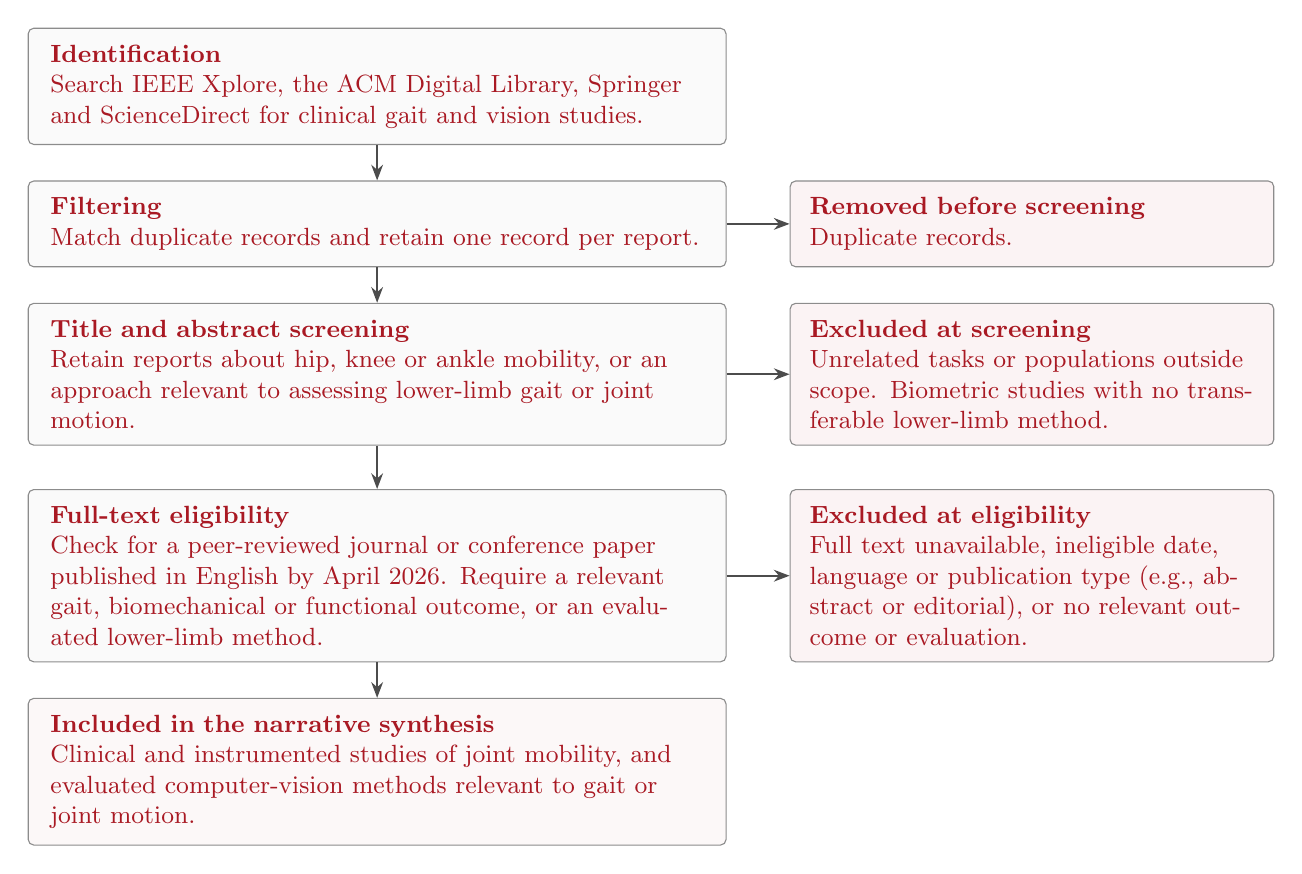
\begin{tikzpicture}[
  stage/.style={
    draw=black!45, fill=black!2, rounded corners=2pt, text=RevisionRed,
    text width=8.3cm, align=left, inner xsep=8pt, inner ysep=6pt, font=\small
  },
  excluded/.style={
    draw=black!45, fill=RevisionRed!5, rounded corners=2pt, text=RevisionRed,
    text width=5.65cm, align=left, inner xsep=7pt, inner ysep=6pt, font=\small
  },
  next/.style={-{Stealth[length=2mm]}, semithick, draw=black!70}
]
\node[stage] (identification) {
  \textbf{Identification}\\
  Search IEEE Xplore, the ACM Digital Library, Springer and ScienceDirect for clinical gait and vision studies.
};
\node[stage, below=4.5mm of identification] (deduplication) {
  \textbf{Filtering}\\
  Match duplicate records and retain one record per report.
};
\node[excluded, right=8mm of deduplication] (duplicates) {
  \textbf{Removed before screening}\\
  Duplicate records.
};
\node[stage, below=4.5mm of deduplication] (screening) {
  \textbf{Title and abstract screening}\\
  Retain reports about hip, knee or ankle mobility, or an approach relevant to assessing lower-limb gait or joint motion.
};
\node[excluded, right=8mm of screening] (offtopic) {
  \textbf{Excluded at screening}\\
  Unrelated tasks or populations outside scope. Biometric studies with no transferable lower-limb method.
};
\node[stage, below=5.5mm of screening] (eligibility) {
  \textbf{Full-text eligibility}\\
  Check for a peer-reviewed journal or conference paper published in English by April 2026. Require a relevant gait, biomechanical or functional outcome, or an evaluated lower-limb method.
};
\node[excluded, right=8mm of eligibility] (ineligible) {
  \textbf{Excluded at eligibility}\\
  Full text unavailable, ineligible date, language or publication type (e.g., abstract or editorial), or no relevant outcome or evaluation.
};
\node[stage, fill=RevisionRed!3, below=4.5mm of eligibility] (included) {
  \textbf{Included in the narrative synthesis}\\
  Clinical and instrumented studies of joint mobility, and evaluated computer-vision methods relevant to gait or joint motion.
};
\draw[next] (identification.south) -- (deduplication.north);
\draw[next] (deduplication.south) -- (screening.north);
\draw[next] (screening.south) -- (eligibility.north);
\draw[next] (eligibility.south) -- (included.north);
\draw[next] (deduplication.east) -- (duplicates.west);
\draw[next] (screening.east) -- (offtopic.west);
\draw[next] (eligibility.east) -- (ineligible.west);
\end{tikzpicture}
\caption{\revred{Screening and selection of studies for the narrative synthesis. The branches show where duplicate, out-of-scope or ineligible records were removed.}}
\label{fig:screening}
\end{figure}


\subsection{\revred{Screening and Selection Procedure}}
\label{sec:screening}
\begin{redrevision}
We removed duplicate records before screening titles and abstracts for relevance. The available full texts were then assessed against the eligibility rules. Figure~\ref{fig:screening} shows the decisions at each stage. It presents the selection rules because database exports and counts for the individual stages were unavailable for reconstruction.
\end{redrevision}



\subsection{\revred{Classification of the Literature}}
\label{sec:classification}
\begin{redrevision}
Figure~\ref{joint_mobility_taxonomy} shows the two evidence groups used in the synthesis. Clinical and instrumented studies help identify the gait variables that matter for hip, knee and ankle mobility. The computer vision studies are discussed by task, including action recognition, video gait analysis and pose estimation. We consider whether a study tests a method on a gait measure or clinical outcome, or whether it provides a technique that could be transferred to joint assessment.

Across both groups, we compare the joint and gait variable, the participant group, recording setup, method, outcome and validation setting. Where a study uses a reference measure or clinical label, we consider what that comparison supports. Agreement with motion capture provides evidence about the accuracy of an angle under the conditions tested. Clinical labels and an appropriate patient sample are needed for a claim about a disorder or its severity. Section~\ref{sec:KO} brings these distinctions together.
\end{redrevision}

\begin{figure}[!htbp]
\centering
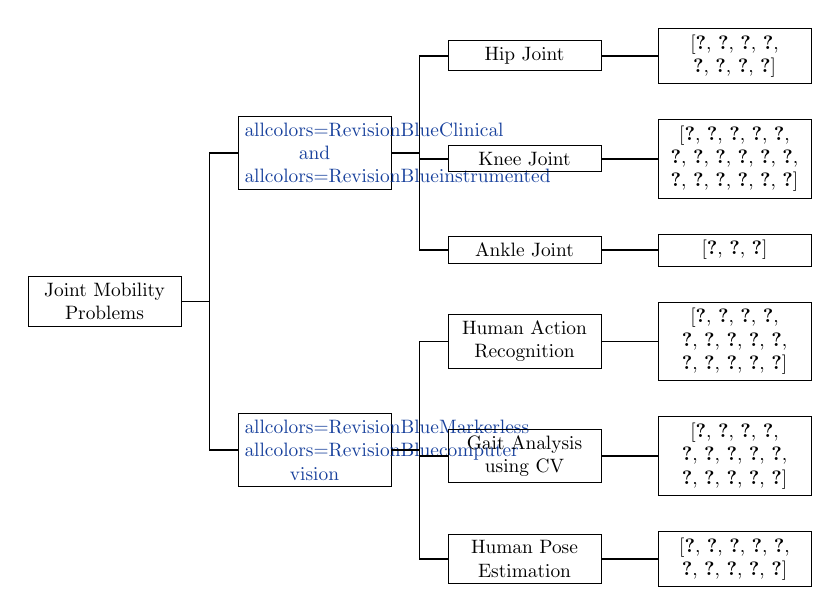
\begin{tikzpicture}[level distance=1.5in, sibling distance=.25in, scale=0.7]
\tikzset{
    edge from parent/.style={thick, draw, edge from parent fork right},
    every tree node/.style={draw, minimum width=0.5in, text width=1in, align=center},
    grow'=right
}
\Tree 
[.{Joint Mobility Problems} 
    [.{\rev{Clinical and}\\ \rev{instrumented}}
        [.{Hip Joint} 
            [.\cite{kiss2010effect,shakoor2003asymmetric,ismailidis2021kinematic,laroche2014classification,meyer2015biomechanical,reininga2012subjects,eitzen2012sagittal,mont2007gait} ]
        ]
        [.{Knee Joint} 
            [.\cite{simonsen2012gait,bejek2006influence,kiss2011effect,elbaz2014novel,bacon2022relation,qingguang2015gait,ro2019effects,butler2009gait,harding2012body,da2012biomechanical,kaufman2001gait,weidow2006hip,favre2016gait,phinyomark2016gender,bkaczkowicz2018gait,astephen2008biomechanical,mcclelland2007gait} ]
        ]
        [.{Ankle Joint} 
            [.\cite{reilly2009role,valderrabano2007gait,schmitt2015effect} ]
        ]
    ]
    [.{\rev{Markerless}\\ \rev{computer vision}}
        [.{Human Action\\ Recognition}
            [.\cite{rohan2020human,vemulapalli2014human,li2010action,boswell2021neural,vafadar2021novel,caetano2019skeleton,suhendar2022skeletal,yadav2022skeleton,ke2017skeletonnet,wang2012mining,ahad2021action,uddin2011human,du2015hierarchical,ahmad2019action} ]
        ]
        [.{Gait Analysis\\ using CV} 
            [.\cite{lv2022analysis,ju1996cardboard,leightley2016automated,fan2020gaitpart,cotton2022transforming,prakash2018vision,uccheddu2022rgb,armstrong2022novel,juri2020characterization,ong2017efficacy,blasco2024computer,wang2024markerless,stenum2024clinical,schoenwether2025reliability} ]
        ]
        [.{Human Pose\\ Estimation} 
            [.\cite{ma2022wushu,li2020human,sharma2022surya,viswakumar2019human,stenum2021two,van2023accuracy,sheu2023improvement,marusic2023evaluating,doong2025predicting,yan2025efficient} ]
        ]
    ]
]
\end{tikzpicture}
\caption{\revred{Classification of the clinical and computer vision literature. The citations give examples of each group. Section~\ref{sec:KO} distinguishes clinical validation from evidence about transferable methods.}}
\label{joint_mobility_taxonomy}
\end{figure}


\subsection{\revred{Supporting Material and Traceability}}
\label{sec:supplement_traceability}
\begin{redrevision}
Supplementary Material S1--S3 gives the individual hip, knee and ankle studies. Sections S4--S6 describe the action recognition, video gait and pose estimation studies, and S7 gives the extended method and benchmark comparisons. The tables retain each study's population, setup, outcome and reported result where available. Results can thus be traced to their original study and interpreted in light of its design.
\end{redrevision}



\section{\rev{Clinical Background and Review Positioning}}
\label{sec:JMP}
\subsection{\rev{Joint Mobility and Gait Variables}}
JMPs refer to a broad class of disorders in which the normal range, smoothness, or coordination of joint movement is compromised due to musculoskeletal, neurological, inflammatory, traumatic, or degenerative causes \cite {pandey2022movement}. These impairments may affect one or multiple joints, most commonly the hip, knee, and ankle in the context of locomotion, and they frequently manifest as pain, stiffness, weakness, instability, compensatory movement, and reduced functional independence \cite{lu2026musculoskeletal,hertling2006management}. Because human walking is a highly coordinated motor activity that depends on the synchronized interaction of lower-limb joints, muscles, and neural control, even subtle alterations in joint mobility can disturb gait mechanics and progressively degrade mobility, balance, and quality of life \cite{yoo2022assessment,hulleck2022present}. For this reason, gait analysis has become a clinically important approach for the objective assessment of JMPs, as it provides quantitative evidence of how joint dysfunction influences spatio-temporal, kinematic, and kinetic characteristics of walking \cite{prakash2018recent,ornetti2010gait}.

\begin{figure} 
    \centering
    \includegraphics[width=\linewidth]{Images/gait_finalized.pdf}
    \caption{Gait cycle representation.}
    \label{fig:gait_cycle}
\end{figure}

The clinical relevance of JMP assessment is particularly evident in disorders such as hip osteoarthritis, knee osteoarthritis, ankle osteoarthritis, generalized joint hypermobility, ligament injury, and post-surgical recovery, where altered gait is both a symptom and a functional biomarker of disease progression \cite{al2002study,bejek2006influence,simonsen2012gait,valderrabano2007gait,mcclelland2007gait}. Figure \ref{fig:gait_cycle} illustrates the gait cycle, which provides the biomechanical framework within which abnormalities can be characterized through parameters such as walking speed, stride length, cadence, temporal asymmetry, joint range of motion, and loading distribution. These parameters are clinically meaningful because they reveal not only the presence of impairment, but also its severity, compensatory adaptations, and response to intervention \cite{andriacchi2006role,baliunas2002increased,kumar2013knee,favre2016gait,bacon2022relation}. In knee osteoarthritis, for example, reductions in speed and stride length, altered knee moments, and abnormal loading patterns are strongly associated with pain and structural degeneration \cite{kaufman2001gait,heiden2009knee,elbaz2014novel}. Similarly, hip pathology may induce asymmetric loading and compensatory trunk movement, while ankle disorders can alter plantar flexion, joint power, and whole-limb walking mechanics \cite{shakoor2003asymmetric,reininga2012subjects,reilly2009role,schmitt2015effect}. Thus, JMPs should not be interpreted as isolated joint-level dysfunctions alone, but rather as system-level disturbances affecting the integrated mechanics of gait.

\begin{figure} 
        \centering
        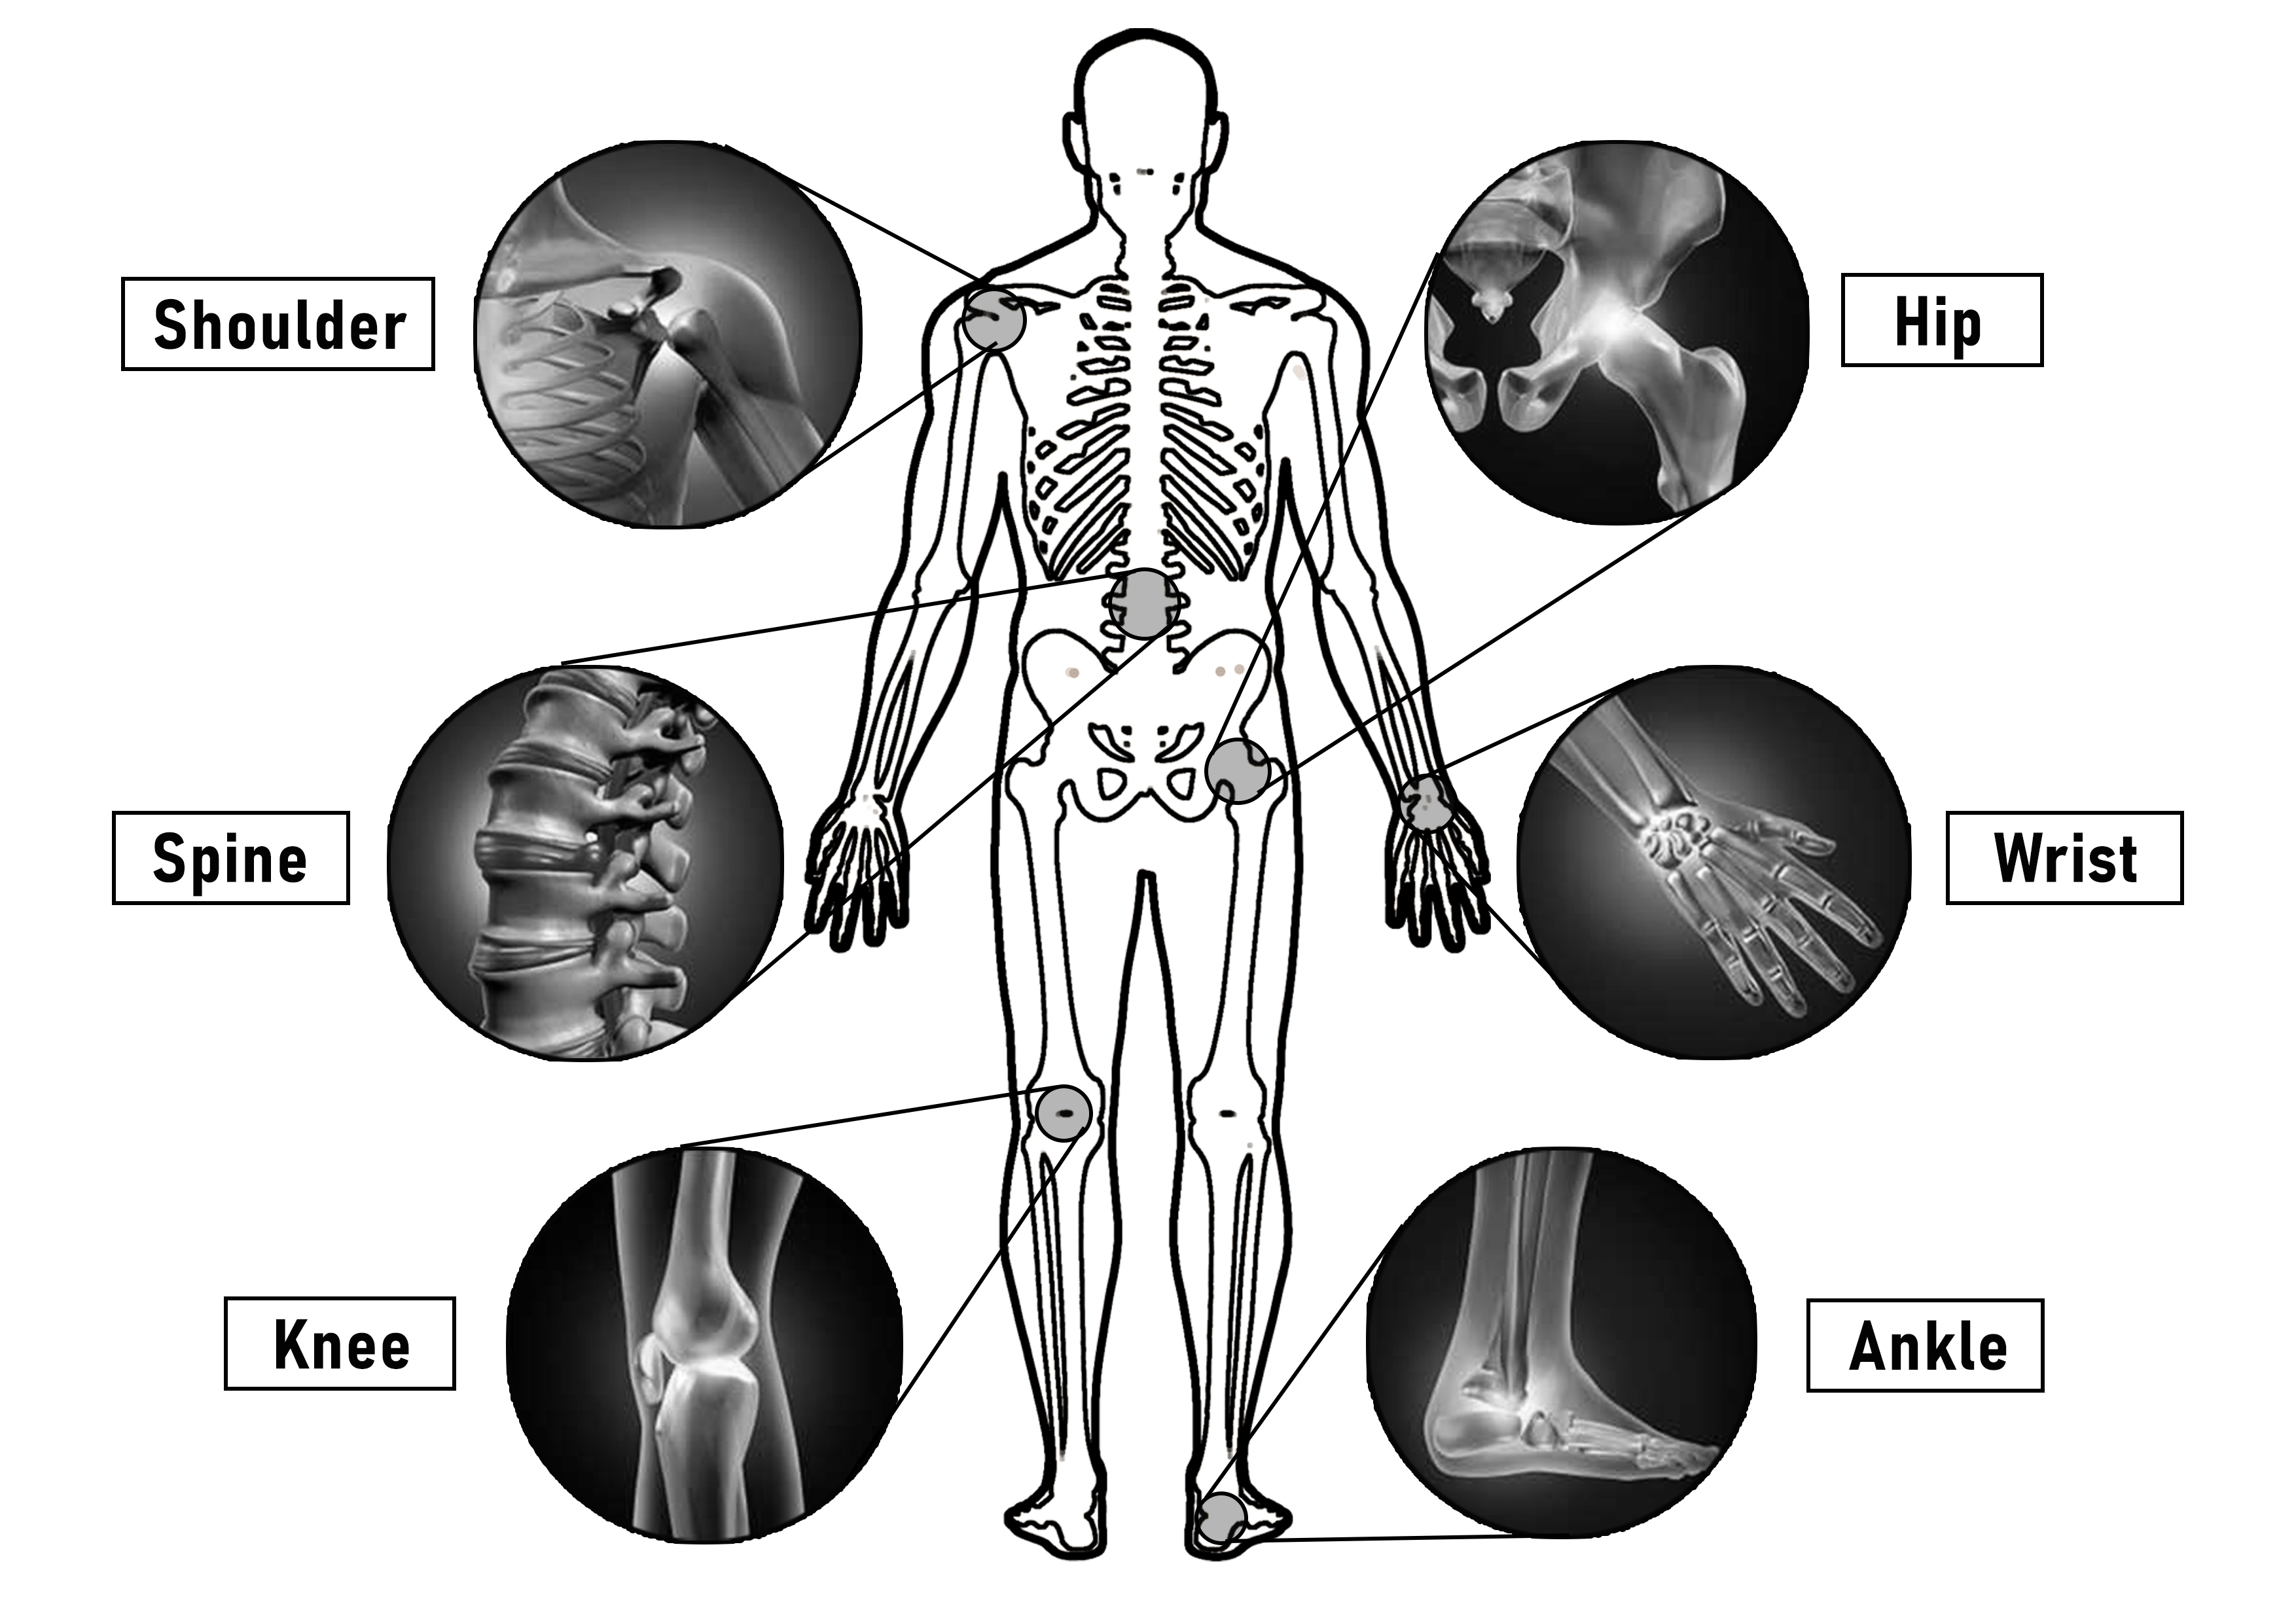
\includegraphics[width=0.6\linewidth]{Images/joint_problems.jpg}
        \caption{Joint mobility problems in human body.}
        \label{Joint Mobility Problems in Human Body}
\end{figure}

Figure \ref{Joint Mobility Problems in Human Body} conceptually illustrates the anatomical distribution of joint mobility problems in the human body. Although JMPs can affect multiple regions, the hip, knee, and ankle are particularly important for gait analysis because they jointly determine limb advancement, shock absorption, load transfer, and postural stability during walking. Figure \ref{jointAngles} further highlights the extension and flexion angles of these lower-limb joints, emphasizing the biomechanical importance of sagittal-plane motion in assessing functional mobility. Abnormalities in these angular patterns are commonly used to identify restricted range of motion, excessive compensation, and pathological gait strategies in patients with joint disorders \cite{astephen2008biomechanical,meyer2015biomechanical,ismailidis2021kinematic}. From a clinical perspective, assessment of these joint-specific deviations can support diagnosis, treatment selection, rehabilitation planning, and post-intervention monitoring.

\begin{figure} 
    \centering
    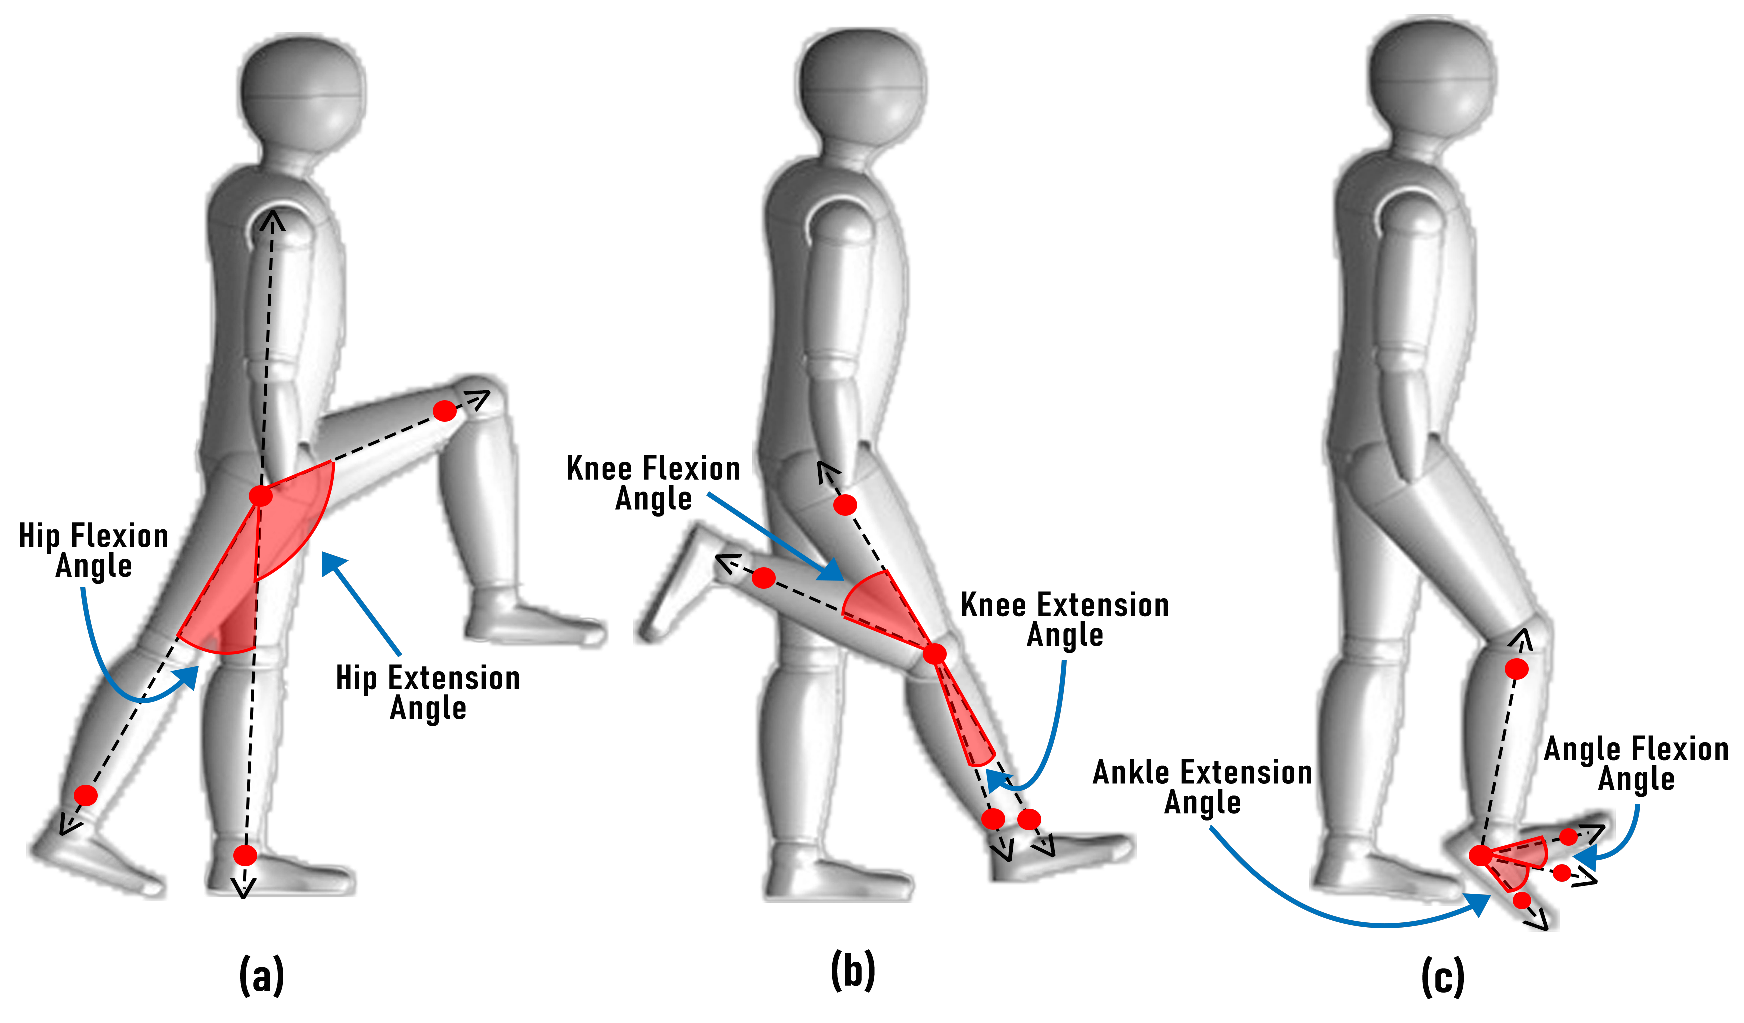
\includegraphics[width=0.6\linewidth]{Images/angles.pdf}
    \caption{Side view angle of human posture showing the extension and flexion angles of the (a) Hip range of motion, (b) Knee joint, and (c) Ankle joint.}
    \label{jointAngles}
\end{figure}

From an application standpoint, computer vision offers several promising pathways for the management of joint mobility disorders. First, gait analysis from video can be used to detect abnormal movement patterns by tracking joint trajectories and comparing them against normative or disease-specific biomechanics \cite{rohan2020human,lv2022analysis,stenum2021two}. Second, vision-based systems can assist rehabilitation by monitoring exercise quality, measuring range of motion, and providing real-time feedback during therapy \cite{debnath2022review,li2020human,uccheddu2022rgb}. Third, marker-less motion analysis can complement pre-operative planning and post-operative monitoring by generating interpretable movement descriptors without the burden of laboratory instrumentation \cite{armstrong2022novel,schoenwether2025reliability}. More broadly, these systems have potential for continuous tracking through low-cost cameras, portable devices, and smart healthcare platforms, thereby extending assessment beyond episodic hospital visits into everyday environments \cite{wang2024markerless,blasco2024computer,doong2025predicting}. Such developments are particularly important for chronic joint conditions, where disease progression and recovery are gradual and require repeated, objective evaluation.


At the same time, the interpretation of JMPs requires more than the detection of isolated visual abnormalities. Pathological gait emerges from the interaction of multiple factors, including joint degeneration, pain avoidance, muscle weakness, compensatory postures, body mass index, and rehabilitation status \cite{harding2012body,gaudreault2011effects,butler2009gait,phinyomark2016gender}. Therefore, robust assessment of JMPs should integrate temporal gait dynamics, joint kinematics, kinetic surrogates, anatomical landmarks, and clinical context. This is why the present survey frames JMP analysis as a progression from traditional clinical gait biomechanics to modern information-rich, vision-based frameworks capable of supporting early diagnosis, objective monitoring, and clinician-friendly decision support. The taxonomy shown in the tree diagram (Figure~\ref{joint_mobility_taxonomy}) further reflects this evolution by distinguishing classical non-computer-vision studies on hip, knee, and ankle pathology from contemporary computer-vision pipelines involving human action recognition, gait analysis, and human pose estimation. Taken together, these developments indicate that the study of joint mobility problems is moving toward a more scalable, interpretable, and translational paradigm in which marker-less vision systems can complement established biomechanical assessment and help bridge the gap between laboratory precision and real-world clinical usability.

\subsection{\rev{Positioning of this Review}}
\label{sec:review_positioning}
\begin{revision}
The closest comparisons are reviews of clinical gait analysis and reviews of the agreement between markerless and marker-based systems. Sethi et al. \cite{sethi2022comprehensive} review gait parameters and measurement methods, including the role of pose estimation in clinical gait analysis. Scataglini et al. \cite{scataglini2024accuracy} compare the accuracy, validity and reliability of three-dimensional gait measurement systems. Hulleck et al. \cite{hulleck2022present} discuss how clinical gait measures and scales are used, while Debnath et al. \cite{debnath2022review} examine computer vision across a wider range of rehabilitation and movement assessment tasks.

This review brings those questions together at the level of a joint and an intended use. It first asks which gait variables matter for hip, knee and ankle mobility, including changes at neighbouring joints. It then asks whether a video method measures the variable, recognises a pattern or supports an inference about a patient's condition. For example, a study that checks knee flexion angles against motion capture can inform measurement in the settings tested. Estimating the severity of knee impairment also requires evidence from patients assessed with a relevant clinical measure. Table~\ref{ExistingSurvey} shows where this emphasis overlaps with earlier reviews and what it adds for joint mobility assessment.
\end{revision}

\begin{table}[!ht]
\centering\small
\caption{\rev{Positioning relative to representative reviews of gait, measurement and movement analysis.}}
\label{ExistingSurvey}
\color{RevisionBlue}\hypersetup{allcolors=RevisionBlue}
\renewcommand{\arraystretch}{1.07}
\begin{tabularx}{0.98\linewidth}{@{}>{\raggedright\arraybackslash}p{0.24\linewidth}>{\raggedright\arraybackslash}p{0.31\linewidth}>{\raggedright\arraybackslash}X@{}}
\toprule
\textbf{Review} & \textbf{Main question or scope} & \textbf{How the present review uses or extends it} \\
\midrule
Sethi et al. \cite{sethi2022comprehensive} & Gait parameters, marker-based and markerless analysis, and pose estimation in clinical gait. & Follows a particular hip, knee or ankle variable from a clinical observation to its video estimate and interpretation. \\ \addlinespace[3pt]
Scataglini et al. \cite{scataglini2024accuracy} & Accuracy, validity and repeatability of three-dimensional markerless gait systems against marker-based systems. & Uses measurement evidence to judge individual variables and extends the comparison to video-based pattern recognition and clinical assessment. \\ \addlinespace[3pt]
Prakash et al. \cite{prakash2018recent} and Hulleck et al. \cite{hulleck2022present} & Gait assessment technologies and applications, including clinical measures, pathology and scales. & Uses the clinical findings to identify which variables and reference measurements matter for a particular joint and task. \\ \addlinespace[3pt]
Debnath et al. \cite{debnath2022review} & Computer vision for physical rehabilitation and movement assessment. & Examines how visual measures of walking relate to lower-limb joint impairment and compensation. \\ \addlinespace[3pt]
Lee et al. \cite{lee2014comprehensive}, Singh et al. \cite{singh2018vision}, Connor and Ross \cite{connor2018biometric}, Isaac et al. \cite{isaac2019trait} (preprint), Khan et al. \cite{khan2021vision}, Sepas-Moghaddam and Etemad \cite{sepas2022deep} & Gait sensing and representations for identifying people. & Draws on representation methods and evaluates their relevance to an explicitly defined mobility variable or outcome. \\ \addlinespace[3pt]
Saboor et al. \cite{saboor2020latest} & Wearable sensing and machine learning for gait analysis. & Places wearable measurements alongside video where they supply a reference or additional information about movement. \\ \addlinespace[3pt]
Kong and Fu \cite{kong2022human} and Gaya-Morey et al. \cite{gaya2024deep} & Action recognition and prediction, activity monitoring and fall detection. & Examines which methods can transfer to joint assessment and what validation of a gait pattern or clinical outcome requires. \\
\bottomrule
\end{tabularx}
\end{table}

\begin{revision}
The contribution is a joint-specific reading of the evidence. The review connects clinical gait findings to candidate video measures in Table~\ref{tab:joint_targets} and shows how the validation requirements change with the intended claim in Table~\ref{tab:validation_claims}. This helps readers judge when a study supports measurement, when it supports recognition of a pattern, and when a clinical conclusion still needs to be tested.
\end{revision}
\FloatBarrier


\section{Joint Mobility Problem as a Computer Vision Task}
\label{sec:JMPCV}

Let
\[
\mathcal{D}=\{(V_i,y_i)\}_{i=1}^{N}
\]
denote a dataset of \(N\) labelled monocular video sequences, where \(V_i\) is the \(i\)-th video and \(y_i\) is its corresponding mobility label. Each video is represented as
\[
V_i=\{f_i^{(t)}\}_{t=1}^{T_i},
\]
where \(f_i^{(t)} \in \mathbb{R}^{H \times W \times C}\) denotes the \(t\)-th RGB frame of the \(i\)-th sequence, \(T_i\) is the number of frames, and \(H\), \(W\), and \(C\) represent the frame height, frame width, and number of channels, respectively. Let
\[
\mathcal{Y}=\{1,2,\ldots,C_m\}
\]
denote the label space of joint mobility conditions, where \(C_m\) is the total number of classes. In the binary case, \(\mathcal{Y}=\{0,1\}\), where \(0\) and \(1\) denote normal and impaired mobility, respectively; in the multiclass case, each class corresponds to a clinically meaningful mobility category.

For each frame \(f_i^{(t)}\), a pose estimation operator
\[
\Psi: \mathbb{R}^{H \times W \times C} \rightarrow \mathbb{R}^{J \times d_k}
\]
extracts a set of \(J\) anatomical body keypoints:
\[
K_i^{(t)}=\Psi(f_i^{(t)})=\{k_{i,j}^{(t)}\}_{j=1}^{J},
\]
where \(k_{i,j}^{(t)} \in \mathbb{R}^{d_k}\) denotes the \(j\)-th body landmark in frame \(t\). For 2D pose estimation, \(d_k=2\); for 3D pose estimation, \(d_k=3\). In the 3D case,
\[
k_{i,j}^{(t)}=\bigl(x_{i,j}^{(t)},y_{i,j}^{(t)},z_{i,j}^{(t)}\bigr).
\]
The temporal pose sequence for the \(i\)-th video is then defined as
\[
K_i=\{K_i^{(t)}\}_{t=1}^{T_i}.
\]

A gait representation function
\[
\Phi: \{K_i^{(t)}\}_{t=1}^{T_i} \rightarrow X_i
\]
maps the pose sequence to a temporal biomechanical feature matrix
\[
X_i \in \mathbb{R}^{T_i \times d},
\]
where \(d\) denotes the number of gait descriptors. These descriptors may encode joint-angle dynamics, limb coordination, symmetry characteristics, and spatio-temporal gait properties. Finally, a classifier
\[
\mathcal{C}: \mathbb{R}^{T_i \times d} \rightarrow \mathcal{Y}
\]
predicts the mobility class label \(\hat{y}_i\).

$-$\noindent\textbf{Mathematical Formulation.}
The joint mobility problem is formulated as a computer vision problem that seeks to infer clinically meaningful mobility status from a monocular gait video. Formally, the objective is to learn a mapping
\[
\mathcal{F}: \mathcal{V} \rightarrow \mathcal{Y},
\]
where \(\mathcal{V}\) denotes the space of video sequences and \(\mathcal{Y}\) denotes the target mobility label space. For a given input video \(V_i\), the prediction is written as
\[
\hat{y}_i=\mathcal{F}(V_i).
\]

In a structured vision pipeline, this mapping is decomposed into three successive stages:
\[
V_i \xrightarrow{\Psi} K_i \xrightarrow{\Phi} X_i \xrightarrow{\mathcal{C}} \hat{y}_i.
\]
That is, the raw video \(V_i\) is first transformed into a sequence of anatomical keypoints \(K_i\), then converted into a discriminative biomechanical representation \(X_i\), and finally classified into one of the mobility categories.

Equivalently, the overall prediction function can be expressed as
\[
\hat{y}_i=\mathcal{C}\bigl(\Phi(\Psi(V_i))\bigr).
\]

Given the labelled dataset \(\mathcal{D}\), the learning objective is to estimate the model parameters \(\theta\) of the predictor \(\mathcal{F}_\theta\) by minimizing the empirical risk:
\[
\theta^\ast=\arg\min_{\theta}\frac{1}{N}\sum_{i=1}^{N}\mathcal{L}\bigl(\mathcal{F}_\theta(V_i),y_i\bigr),
\]
where \(\mathcal{L}(\cdot,\cdot)\) denotes a suitable classification loss function, such as binary cross-entropy for two-class mobility assessment or categorical cross-entropy for multiclass mobility classification.

Under this formulation, joint mobility assessment is cast as a fine-grained vision-based human motion understanding problem. Unlike generic action recognition, the task is not merely to identify broad activities such as walking or standing, but rather to detect subtle spatial and temporal deviations in joint movement patterns that reflect mobility impairment. Hence, the problem requires the model to capture: i) anatomically meaningful body structure, ii) temporally evolving gait dynamics, and iii) discriminative biomechanical irregularities associated with impaired motion. This formulation provides the mathematical basis for designing interpretable computer vision systems for automated, non-invasive, and clinically relevant joint mobility analysis.

\begin{revision}
The formulation above applies to classification with a defined set of labels. Estimating a joint angle or walking speed instead requires a continuous target and comparison with a reference measurement. Predicting future falls requires a time horizon and observed follow-up outcomes. A joint moment inferred from video also depends on the model and reference data used to link visible movement to loading. Section~\ref{sec:KO} sets out the corresponding validation requirements.
\end{revision}


\section{\rev{Clinical and instrumented evidence for joint mobility assessment}}
\label{sec:JMPWTCV}
\begin{revision}
Clinical studies identify the gait variables that matter for lower-limb mobility. They also provide reference measurements for judging video-based estimates. The studies considered here use marker-based motion capture, force platforms, wearable sensors or clinical measurements. These include optical systems that track markers fixed to the body. Supplementary Material S1--S3 gives the cohorts, protocols and findings for individual studies.
\end{revision}

\subsection{\rev{Hip joint mobility problems}}
\label{sec:hip_synthesis}
\begin{revision}
The hip literature points to three connected outcomes: restricted motion, altered symmetry and compensation elsewhere in the body. Studies of hip osteoarthritis report reduced hip excursion, changes in late-stance extension and altered pelvic or trunk movement \cite{kiss2010effect,eitzen2012sagittal,reininga2012subjects,ismailidis2021kinematic}. Walking speed must be considered when interpreting these differences. Speed-matched comparisons are particularly useful because some kinematic differences remain after the effect of slower walking is reduced \cite{ismailidis2021kinematic}.

The affected hip is only part of the assessment. Shakoor et al. \cite{shakoor2003asymmetric} report altered loading at the contralateral knee, while Reininga et al. \cite{reininga2012subjects} describe trunk and pelvic compensation. A vision model that tracks only the affected hip could therefore miss clinically relevant adaptations. Classification studies using kinematic trajectories or reduced biomechanical features further show that gait contains information about hip osteoarthritis \cite{laroche2014classification,meyer2015biomechanical}. Their results concern the studied acquisition systems and cohorts; they do not establish equivalent performance from an ordinary camera.

For video-based assessment, hip excursion, bilateral asymmetry and trunk--pelvis motion are reasonable measurement targets. These estimates should be checked against joint-specific reference measurements and interpreted alongside pain and function. Postoperative comparisons also require care: favourable gait findings in selected arthroplasty groups do not establish a general treatment advantage \cite{mont2007gait}. Supplementary Material S1 presents the study-level detail behind this synthesis.
\end{revision}

\subsection{\rev{Knee joint mobility problems}}
\label{sec:knee_synthesis}
\begin{revision}
Knee osteoarthritis studies repeatedly identify changes in walking speed, stride length, knee motion and loading \cite{kaufman2001gait,astephen2008biomechanical,favre2016gait}. The interpretation depends on the question being asked. Spatiotemporal features can support functional classification \cite{elbaz2014novel}; step regularity and related measures can reveal associations with knee pain \cite{bacon2022relation}; and joint moments describe loading that cannot be read directly from a two-dimensional image \cite{baliunas2002increased,andriacchi2006role}. These outcomes should remain separate in a clinical comparison.

Several factors complicate attribution. Speed changes many gait variables, body mass index affects movement and loading, and severity changes gait variability \cite{bejek2006influence,harding2012body,kiss2011effect}. Generalised joint hypermobility and previous ligament reconstruction introduce further movement patterns that are not interchangeable with osteoarthritis \cite{simonsen2012gait,butler2009gait}. Knee pathology also affects neighbouring joints, so hip and ankle motion should be considered when interpreting a knee-focused model \cite{ro2019effects,weidow2006hip}.

The practical implication is that an abnormality classifier should not be interpreted as a severity score unless severity was explicitly labelled and validated. Similarly, a reduction in pain after treatment does not guarantee normalisation of gait. Rehabilitation and arthroplasty studies provide reasons to measure symptoms and movement separately \cite{qingguang2015gait,bkaczkowicz2018gait,mcclelland2007gait}. For vision systems, the most useful progression is from validated step timing and knee-angle trajectories to more demanding loading or severity estimates, with a separate validation for each output. Supplementary Material S2 gives the individual study results and limitations.
\end{revision}

\subsection{\rev{Ankle joint mobility problems}}
\label{sec:ankle_synthesis}
\begin{revision}
The ankle evidence included in this survey is smaller than the hip and knee evidence. It nevertheless shows why distal-joint assessment should not be reduced to walking speed alone. Reilly et al. \cite{reilly2009role} relate foot posture and dorsiflexion to hip and knee osteoarthritis, while Valderrabano et al. \cite{valderrabano2007gait} show that improvements after ankle replacement can coexist with residual differences in plantar flexion, moments or power. Schmitt et al. \cite{schmitt2015effect} further illustrate the effects of lower-limb osteoarthritis across the joint chain.

For a vision system, dorsiflexion and plantar flexion are relevant targets, but they require reliable foot and shank landmarks. A detector that estimates the ankle centre without a stable foot segment cannot be assumed to recover the same angle as a clinical biomechanical model. Joint power and loading require additional modelling or sensing. The limited evidence also argues against transferring knee-validation results directly to the ankle. Supplementary Material S3 discusses the clinical protocols and detailed findings.
\end{revision}

\subsection{\rev{Implications for vision-based measurement}}
\label{sec:joint_measurements}
\begin{revision}
Across the three joints, the key issue is the link between the intended measurement and the clinical interpretation. Table~\ref{tab:joint_targets} summarises that link. A change in walking speed is observable but not specific to one disorder. A joint-angle trajectory is more anatomically informative, but its accuracy depends on landmark definitions, viewing geometry and recording conditions. A kinetic estimate requires an additional model and an appropriate reference. These distinctions provide the basis for assessing the computer-vision literature in the next section.
\end{revision}
{\small\setlength{\tabcolsep}{4pt}\renewcommand{\arraystretch}{1.12}
\begin{table}[!htbp]
\centering\small
\caption{\rev{Joint-specific measurement targets and validation needs identified in the reviewed studies.}}\label{tab:joint_targets}
\begin{tabular}{>{\raggedright\arraybackslash}p{2.4cm}p{4.2cm}p{4.5cm}p{4.5cm}}
\toprule\rev{Joint} & \rev{Clinical gait findings} & \rev{Candidate video measures} & \rev{Required interpretation or validation}\\\midrule
\rev{Hip} & \rev{Restricted excursion; bilateral and trunk--pelvis compensation \cite{eitzen2012sagittal,reininga2012subjects}.} & \rev{Hip-angle trajectories, asymmetry, pelvic and trunk motion.} & \rev{Match angle definitions and speed conditions; assess both limbs and neighbouring segments.}\\\midrule
\rev{Knee} & \rev{Changed flexion, regularity and loading; influence of pain and body mass \cite{bacon2022relation,harding2012body}.} & \rev{Knee-angle trajectories, step timing and regularity; model-based moment estimates.} & \rev{Separate kinematic error from loading prediction; validate severity against an explicit clinical target.}\\\midrule
\rev{Ankle} & \rev{Altered dorsiflexion, plantar flexion, propulsion and compensation \cite{valderrabano2007gait,schmitt2015effect}.} & \rev{Foot--shank angles, timing and bilateral patterns.} & \rev{Validate foot landmarks and motion planes; do not equate angle estimates with force or power.}\\\bottomrule
\end{tabular}
\end{table}}

\FloatBarrier
Table~\ref{tableCV} records the motion planes and analytical methods used in the instrumented studies. Knee motion was examined more often than ankle motion in this set of studies. The range of camera systems, sensors and analytical methods also matters when comparing results across joints.
\begingroup
\footnotesize
\setlength{\tabcolsep}{3.3pt}
\renewcommand{\arraystretch}{1.08}
\begin{longtable}{@{}r >{\raggedright\arraybackslash}p{3.55cm}
    *{6}{c} >{\raggedright\arraybackslash}p{8.55cm}@{}}
\caption{Motion planes and analytical methods used in studies of gait-based joint mobility. K1 and K2 denote sagittal and frontal knee motion, H1 and H2 denote sagittal and frontal hip motion, and A1 and A2 denote sagittal and frontal ankle motion. Y indicates that the study considered the plane.}\label{tableCV}\\
\toprule

\textbf{No.} & \textbf{Author (year)} & \multicolumn{6}{c}{\textbf{Motion planes considered}} & \textbf{Technique and software used} \\
\cmidrule(lr){3-8}
& & \textbf{K1} & \textbf{K2} & \textbf{H1} & \textbf{H2} & \textbf{A1} & \textbf{A2} & \\
\midrule

\endfirsthead
\multicolumn{9}{@{}l}{\textbf{Table \thetable\ continued}}\\[2pt]
\toprule

\textbf{No.} & \textbf{Author (year)} & \multicolumn{6}{c}{\textbf{Motion planes considered}} & \textbf{Technique and software used} \\
\cmidrule(lr){3-8}
& & \textbf{K1} & \textbf{K2} & \textbf{H1} & \textbf{H2} & \textbf{A1} & \textbf{A2} & \\
\midrule

\endhead
\midrule
\endfoot
\bottomrule
\endlastfoot
1. & K. R. Kaufman \cite{kaufman2001gait} (2001) & Y & Y & N & N & N & N & Marker-based 6-camera setup with ADTECH, OrthoTrak, and SAS \\
2. & N. Shakoor \cite{shakoor2003asymmetric} (2003) & Y & Y & N & N & N & N & Marker-based optoelectronic camera setup with two-tailed paired-samples \textit{t}-test \\
3. & Z. Bejek \cite{bejek2006influence} (2006) & Y & Y & Y & Y & N & N & Zebris CMS-HS with Statistica and ANOVA \\
4. & J. Weidow \cite{weidow2006hip} (2006) & Y & Y & Y & Y & N & N & Marker-based 6-camera setup with QTracC, QGait, and SPSS \\
5. & M. A. Mont \cite{mont2007gait} (2007) & N & Y & Y & Y & N & Y & Marker-based 8-camera setup with OrthoTrak \\
6. & J. A. McClelland \cite{mcclelland2007gait} (2007) & Y & Y & N & N & N & N & Checklist for the assessment of methodological quality \\
7. & V. Valderrabano \cite{valderrabano2007gait} (2007) & N & N & N & N & Y & Y & Marker-based 6-camera setup with SF-36, AOFAS, Mathcad, ANOVA, and SPSS \\
8. & J. L. Astephen \cite{astephen2008biomechanical} (2008) & Y & Y & Y & Y & N & Y & Optotrak 3020 optoelectronic motion capture system and WOMAC with one-way ANOVA \\
9. & R. Butler \cite{butler2009gait} (2009) & Y & N & Y & N & N & N & Marker-based 8-camera setup and Visual3D with SPSS \\
10. & K. Reilly \cite{reilly2009role} (2009) & N & N & N & N & N & Y & Goniometric measurement and FPI with SPSS \\
11. & R. M. Kiss \cite{kiss2010effect} (2010) & N & Y & Y & Y & N & N & Zebris CMS-HS with two-factor ANOVA and SPSS \\
12. & R. M. Kiss \cite{kiss2011effect} (2011) & N & Y & Y & Y & N & N & Zebris CMS-HS with SPSS and ANCOVA \\
13. & I. H. Reininga \cite{reininga2012subjects} (2012) & N & N & Y & Y & N & N & Two triaxial sensors with Xsens and SPSS \\
14. & I. Eitzen \cite{eitzen2012sagittal} (2012) & Y & Y & Y & Y & N & Y & Marker-based 8-camera setup with SPSS and WOMAC \\
15. & E. B. Simonsen \cite{simonsen2012gait} (2012) & Y & N & Y & Y & Y & N & Marker-based 5-camera setup with PASW and Ariel APAS \\
16. & G. T. Harding \cite{harding2012body} (2012) & Y & Y & N & N & N & N & Optotrak 3020 motion capture system with MATLAB, PCA, and two-factor ANOVA \\
17. & H. G. da Silva \cite{da2012biomechanical} (2012) & Y & Y & N & N & Y & Y & Marker-based 6-camera setup with SPSS \\
18. & D. Laroche \cite{laroche2014classification} (2014) & Y & Y & Y & Y & Y & Y & Marker-based 8-camera setup with SVM, ROC analysis, and ANOVA \\
19. & A. Elbaz \cite{elbaz2014novel} (2014) & Y & Y & N & N & N & N & WOMAC and SF-36 scores \\
20. & C. A. Meyer \cite{meyer2015biomechanical} (2015) & Y & Y & Y & Y & Y & N & Marker-based 15-camera setup with PCA and LDA \\
21. & Z. Qingguang \cite{qingguang2015gait} (2015) & Y & N & Y & N & Y & N & Marker-based 6-camera setup and WOMAC with SPSS \\
22. & D. Schmitt \cite{schmitt2015effect} (2015) & N & Y & N & Y & N & Y & Marker-based 8-camera setup with 1$\times$4 ANOVA \\
23. & J. Favre \cite{favre2016gait} (2016) & Y & Y & N & N & N & N & Camera-based motion capture system \\
24. & A. Phinyomark \cite{phinyomark2016gender} (2016) & Y & Y & Y & Y & Y & Y & 8-camera VICON motion capture system with 3D Gait, PCA, ANOVA, and SVM \\
25. & D. B{\k{a}}czkowicz \cite{bkaczkowicz2018gait} (2018) & N & N & N & N & N & N & GAITRite force mat and WOMAC with one-way ANOVA and Statistica \\
26. & D. H. Ro \cite{ro2019effects} (2019) & Y & Y & Y & Y & Y & Y & Marker-based 12-camera setup with MATLAB and SPSS \\
27. & P. Ismailidis \cite{ismailidis2021kinematic} (2021) & N & Y & N & Y & N & Y & RehaGait with Hasomed GmbH, MATLAB, and SPSS \\
28. & K. L. Bacon \cite{bacon2022relation} (2022) & Y & Y & N & N & N & N & Marker-based camera setup and WOMAC with SAS and R \\
\end{longtable}
\endgroup


\section{\rev{Vision-based methods for joint mobility assessment}}
\label{sec:JMPWCV}
\begin{revision}
The vision literature is organised here by the role of each method in the assessment pipeline. Human action recognition supplies movement representations and classifiers; gait analysis converts movement into walking-related descriptors; and pose estimation provides the landmarks on which many of those descriptors depend. These categories overlap. A single clinical system may use all three, but evidence for one component does not validate the complete assessment. The detailed descriptions and model comparisons are retained in Supplementary Material S4--S7.
\end{revision}

\begin{figure}  
    \centering
    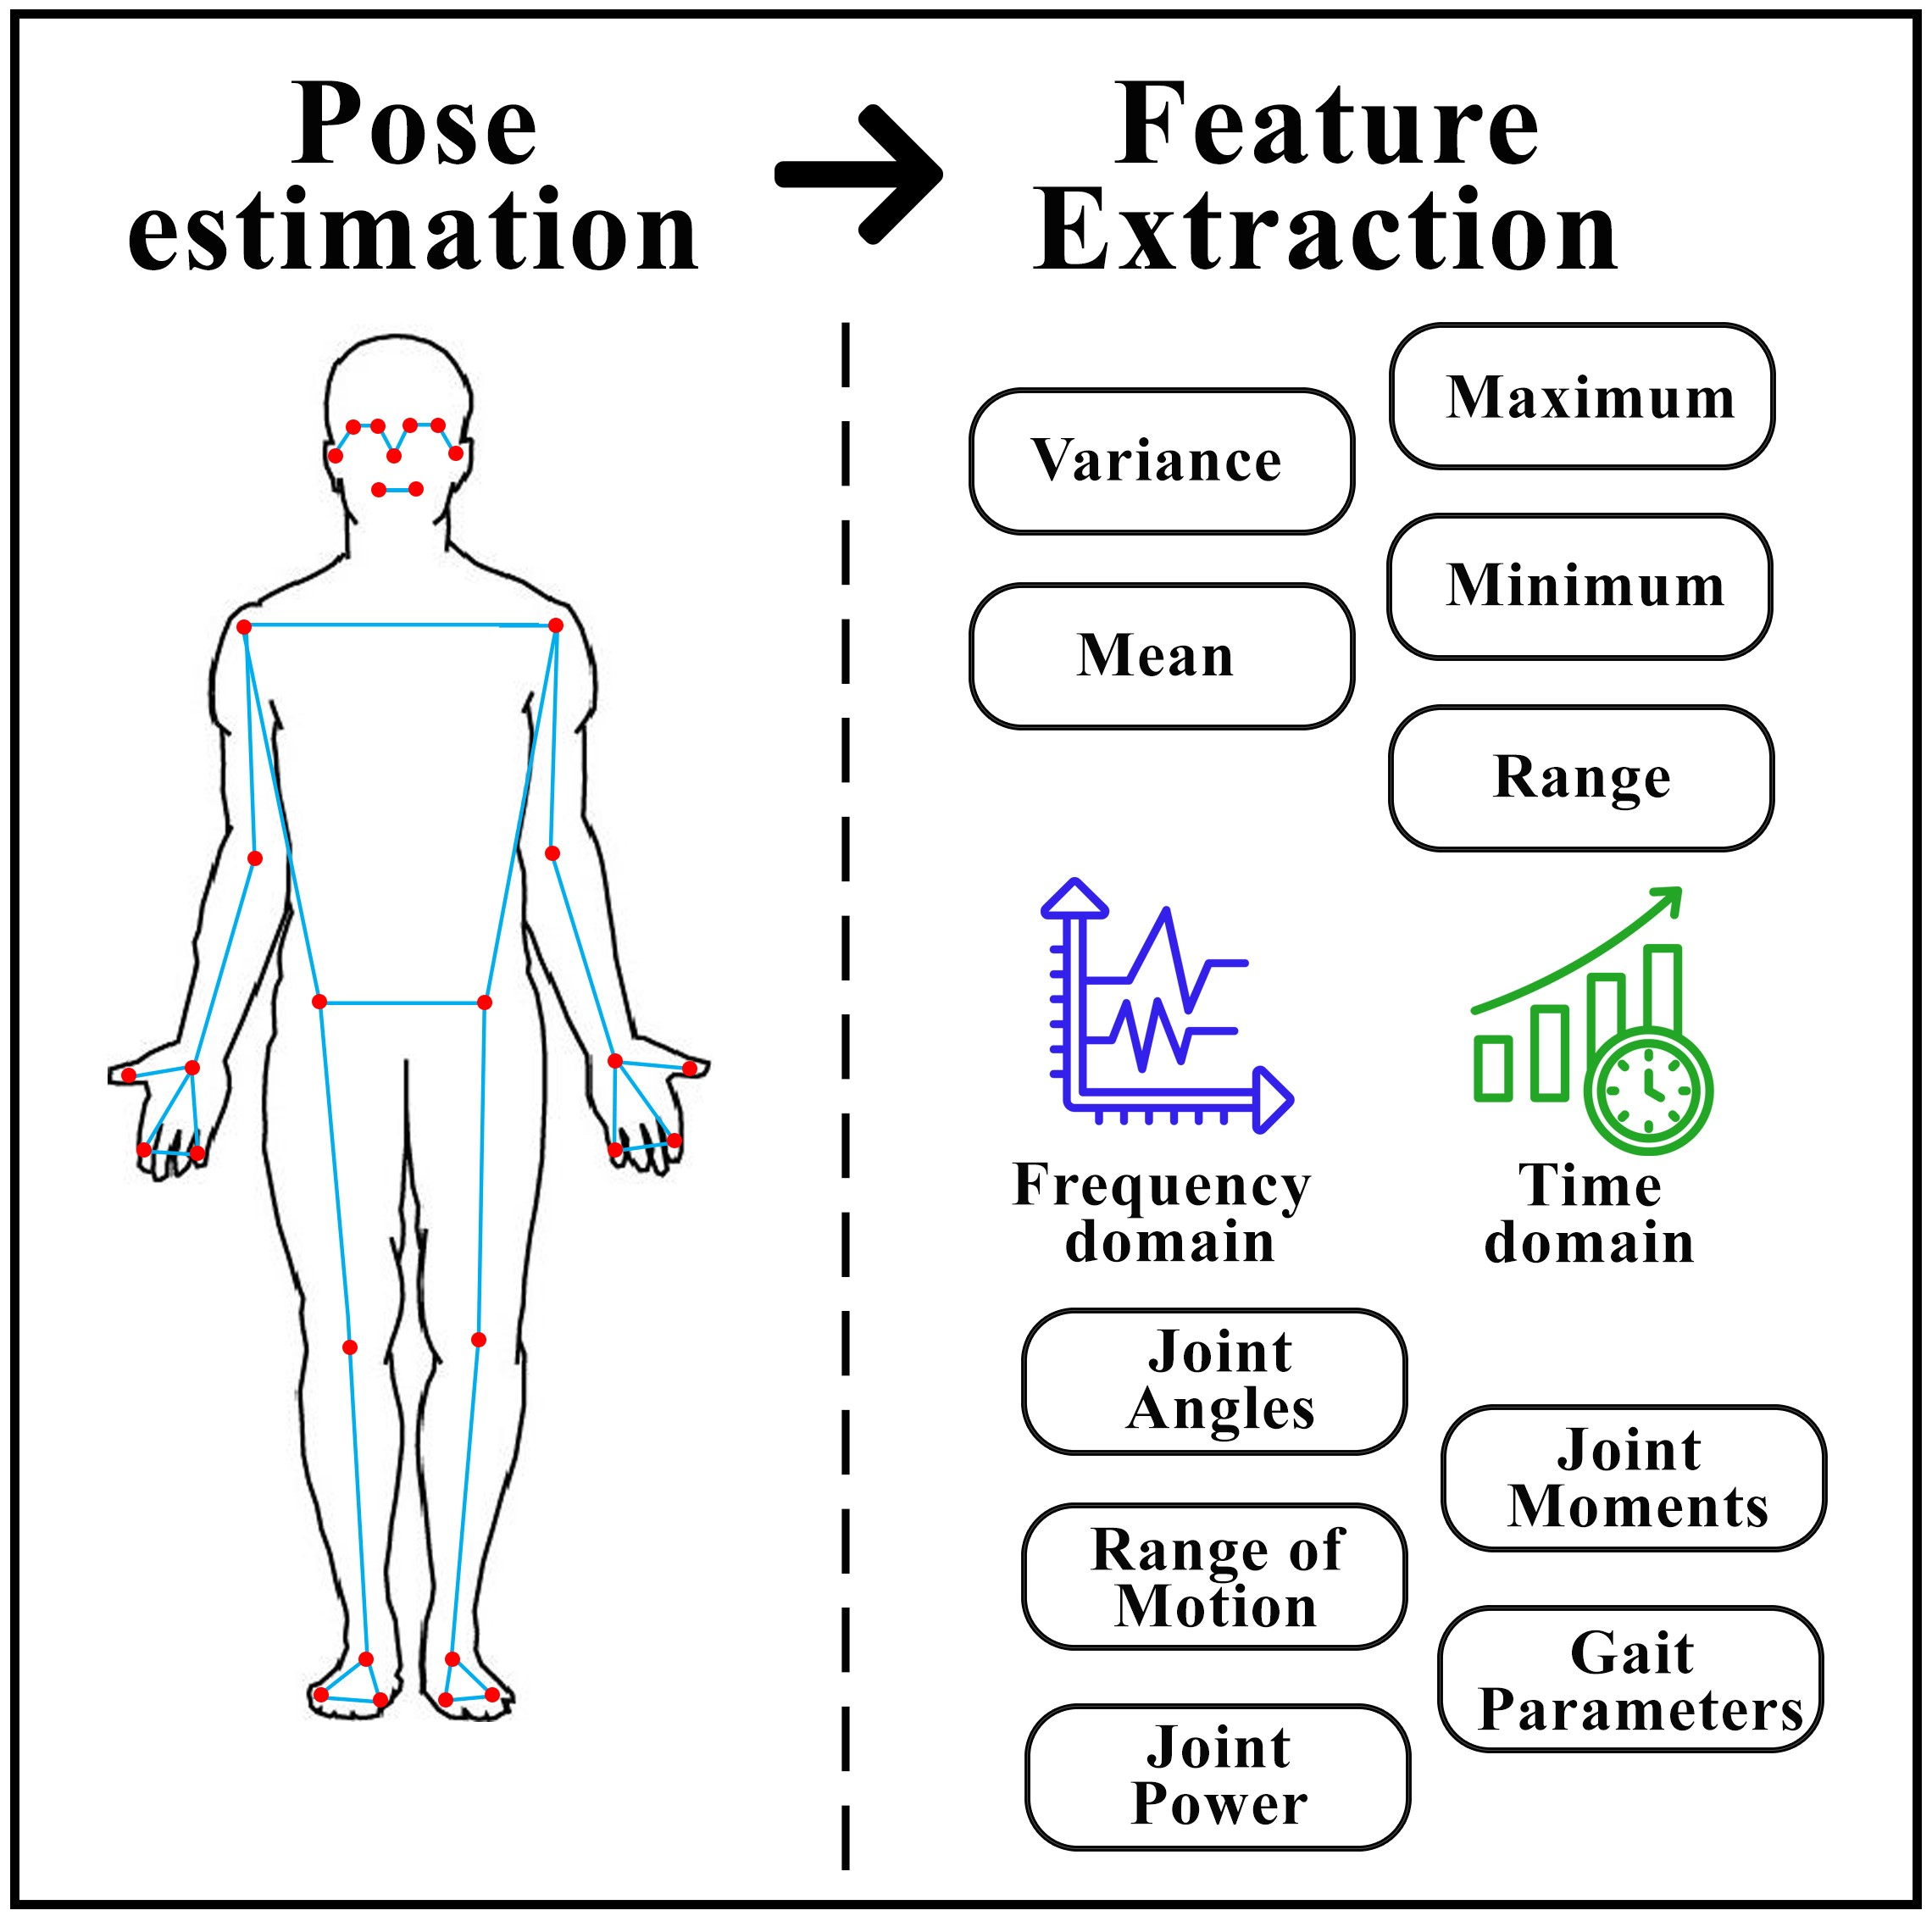
\includegraphics[width=300pt]{Images/mediapipe_figure.jpg}
    \caption{Using HAR for Joint mobility problem.}
    \label{HAR for Joint mobility problem}
\end{figure}

\subsection{\rev{Human action recognition}}
\label{sec:har_synthesis}
\begin{revision}
Skeleton-based human action recognition (HAR) offers several ways to represent movement (Figures~\ref{HAR for Joint mobility problem} and~\ref{Skeleton-based human action recognition}). Lie-group representations encode relationships between body segments, recurrent models capture temporal structure, and graph-based models represent connections between joints \cite{vemulapalli2014human,du2015hierarchical,ahmad2019action}. Skeleton images and kinematic feature sets provide other representations of these relationships \cite{caetano2019skeleton,ke2017skeletonnet,ahad2021action}. These methods are relevant to gait because timing and coordination matter alongside individual poses.

Recognising a walking action on MSR-Action3D or NTU RGB+D tests whether a method can identify a movement. Distinguishing pain-related compensation from a particular joint disorder requires patient data and clinically defined labels. For the same reason, temporal models such as convolutional long short-term memory networks (ConvLSTMs) and transformers need separate evaluation for joint angles, loading or severity \cite{yadav2022skeleton,suhendar2022skeletal}. Supplementary Material S7 gives the action recognition results in their original settings.

Rohan et al. \cite{rohan2020human} use pose-guided learning to recognise abnormal gait patterns. Boswell et al. \cite{boswell2021neural} use two-dimensional projections of motion-capture landmarks to estimate peak knee adduction moment. Their results were stronger for frontal than sagittal projections, indicating that viewpoint matters even with laboratory-derived landmarks. Testing the method with landmarks estimated from actual video is a further step. These two studies illustrate why the validation must match the output, whether a gait label or a biomechanical estimate.

Task-specific training also matters. Vafadar et al. \cite{vafadar2021novel} examine gait-specific data for improving joint localisation, which addresses the mismatch between general pose datasets and walking measurements. For joint-mobility applications, model choice should therefore follow the required outcome and the available clinical labels. Supplementary Material S4 shows the individual architectures, datasets and reported results.
\end{revision}

\begin{figure}
    \centering
    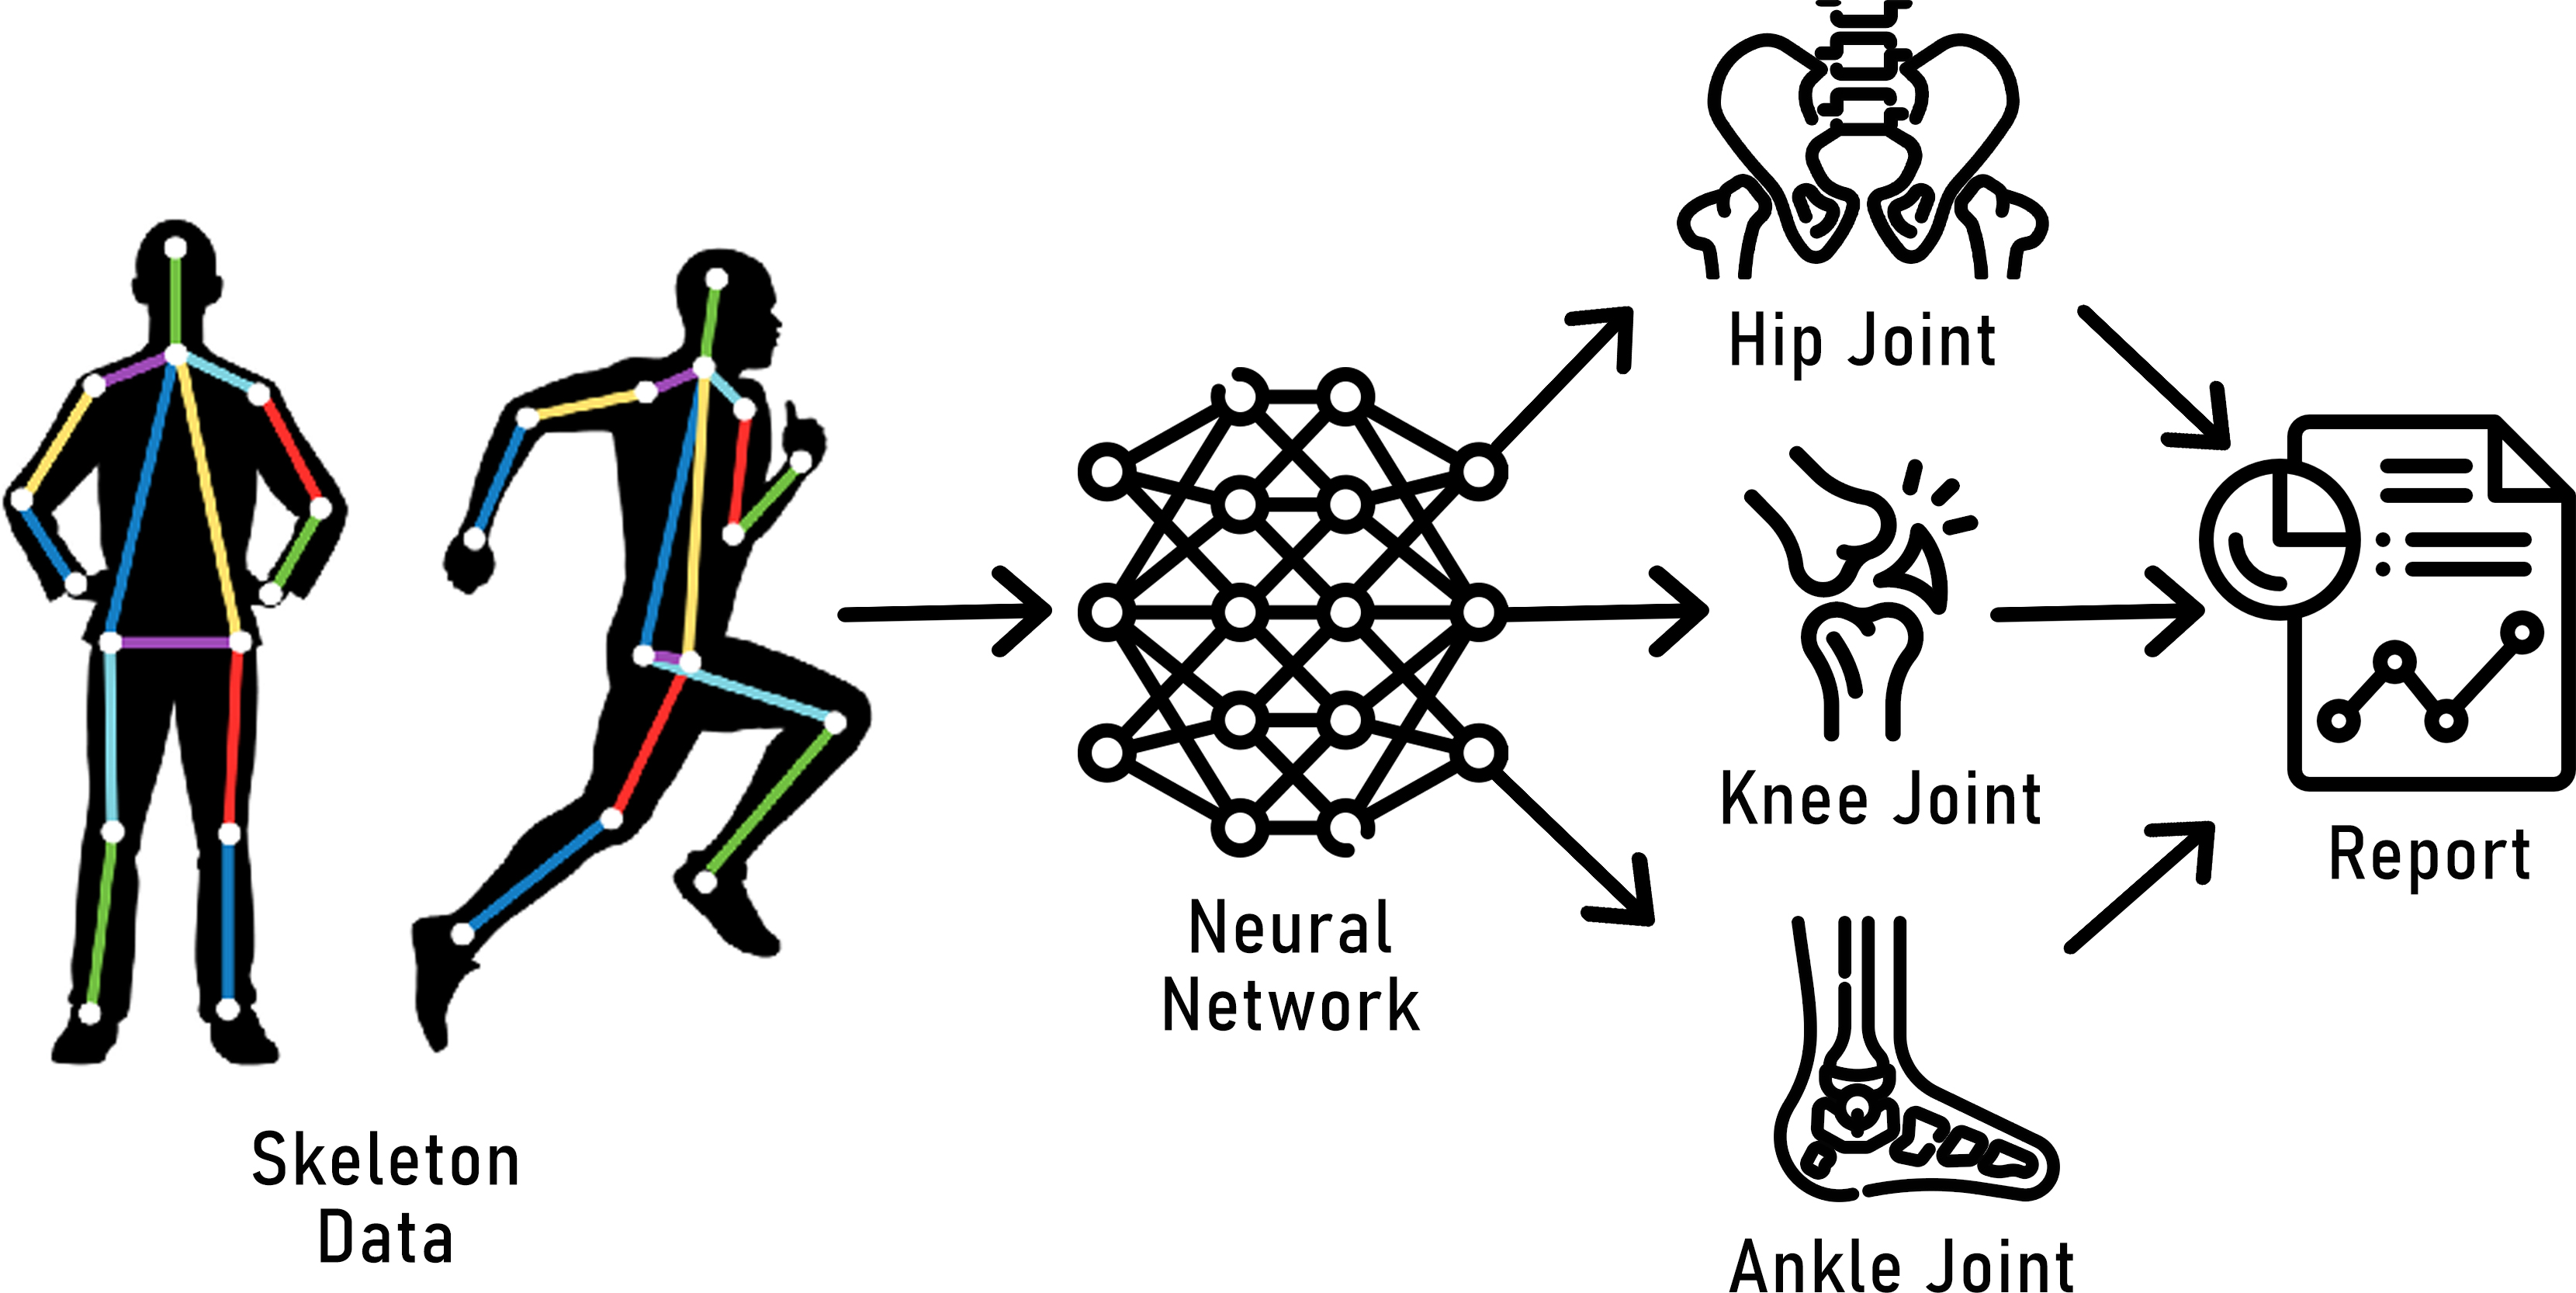
\includegraphics[width=.8\linewidth]{Images/flowchart.jpg}
    \caption{Skeleton-based human action recognition using deep learning model.}
    \label{Skeleton-based human action recognition}
\end{figure}

\subsection{\rev{Gait analysis from video}}
\label{sec:gait_synthesis}
\begin{revision}
Video-based gait analysis includes both direct measurement and learned inference. Geometric methods recover features from silhouettes or landmarks; other methods learn gait descriptors from pose trajectories or image sequences \cite{prakash2018vision,cotton2022transforming}. Lv et al. \cite{lv2022analysis}, for example, combine pose trajectories with entropy-based analysis to distinguish movement patterns associated with knee osteoarthritis. The relevant question is whether a descriptor retains a useful relationship with the clinical variable of interest, rather than whether its representation is more complex.

Validation studies show that results depend on the acquisition setup, joint and motion plane. RGB-D rehabilitation measurements, calibrated markerless tracking and OpenPose-based analysis have been compared with motion capture or inertial references \cite{uccheddu2022rgb,ong2017efficacy,juri2020characterization}. In their review of 3D systems, Scataglini et al. \cite{scataglini2024accuracy} report stronger agreement for spatiotemporal variables than for ankle kinematics. The home setting adds uncertainties about calibration, camera placement and visibility. Armstrong et al. \cite{armstrong2022novel} also show why acquisition burden matters when equipment worn by a participant changes how they walk.

Biometric gait methods offer a useful example of the limits of transfer. GaitPart models local body regions and short-range temporal patterns \cite{fan2020gaitpart}. Such representations may help study localised movement changes, but the reported biometric evaluation does not establish localisation of hip, knee or ankle pathology. Earlier articulated-body models likewise provide a methodological foundation rather than clinical evidence \cite{ju1996cardboard}.

For joint-level assessment, the strongest comparison is an outcome-matched one: estimate the same variable, with the same anatomical convention and gait-cycle definition, and compare it against an appropriate reference. Calibration, camera placement, walking speed and the handling of missing landmarks should be stated. Supplementary Material S5 retains the individual study descriptions, strengths and limitations.
\end{revision}

Table~\ref{gaitapps} shows where individual gait parameters are used in clinical analysis, monitoring and sport. The application determines which measures are relevant. Kinetic quantities such as muscle force require additional sensing or modelling.
\begin{table}[!htbp]
\centering\small
\caption{Gait parameters and application domains.}
\label{gaitapps}
\renewcommand{\arraystretch}{1.07}
\begin{tabularx}{0.94\linewidth}{@{}r >{\raggedright\arraybackslash}X c c c@{}}
\toprule
\textbf{No.} & \textbf{Gait parameter} & \textbf{Clinical analysis} & \textbf{Monitoring system} & \textbf{Sports domain}\\
\midrule
1.  & Body posture & Yes & Yes & Yes \\
2.  & Gait phases & Yes &  & Yes \\
3.  & Step length & Yes & Yes & Yes \\
4.  & Swing time & Yes &  & Yes \\
5.  & Step width & Yes &  &  \\
6.  & Stride length & Yes & Yes & Yes \\
7.  & Stance time & Yes &  &  \\
8.  & Muscle force & Yes &  & Yes \\
9.  & Rhythm & Yes & Yes & Yes \\
10. & Momentum & Yes & Yes & Yes \\
11. & Joint angle & Yes &  & Yes \\
12. & Stride velocity & Yes & Yes &  \\
13. & Knee angle & Yes &  & Yes \\
14. & Ankle Range of Motion (ROM) & Yes &  & Yes \\
15. & Hip ROM & Yes &  & Yes \\
\bottomrule
\end{tabularx}
\end{table}


\begin{figure}  
    \centering
    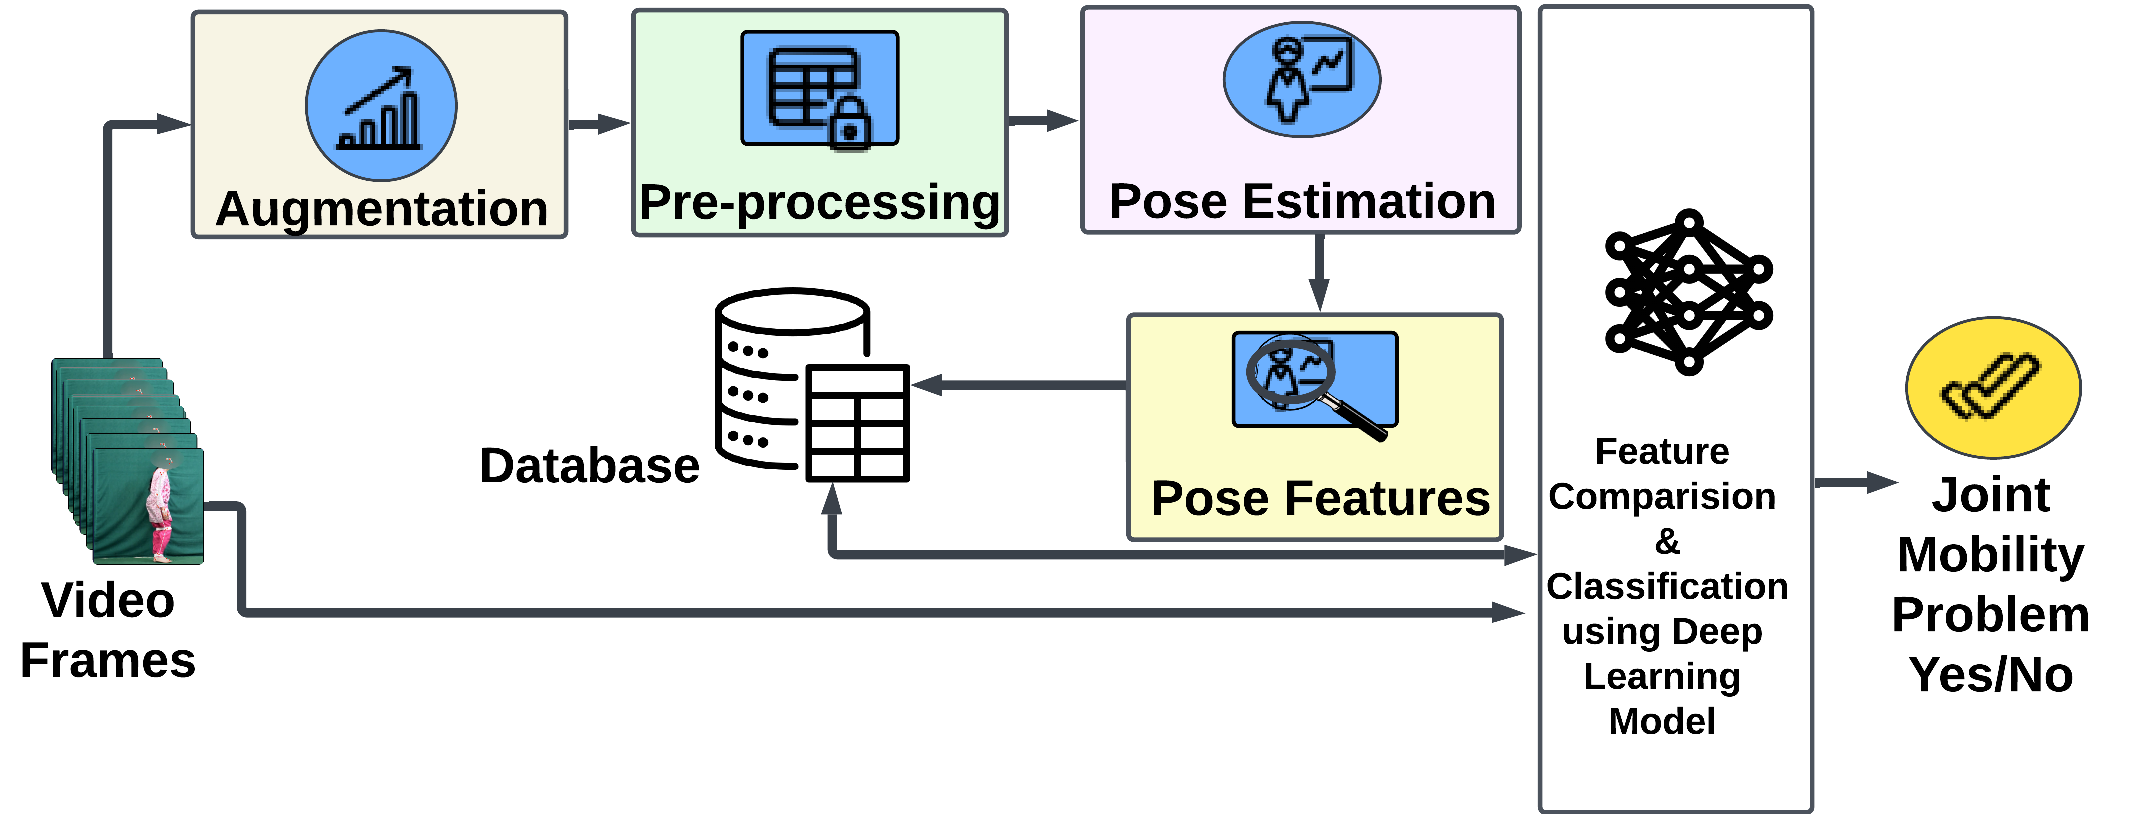
\includegraphics[width=400pt]{Images/Survey_HPE.pdf}
    \caption{Using Human Pose estimation for the Joint mobility problem.}
    \label{HPE_joint mobility problem}
\end{figure}

\subsection{\rev{Human pose estimation}}
\label{sec:hpe_synthesis}
\begin{revision}
Human pose estimation (HPE) supplies the landmark trajectories from which many gait variables are calculated (Figure~\ref{HPE_joint mobility problem}). Stenum et al. \cite{stenum2021two} compared OpenPose estimates with motion capture during overground walking in 31 healthy participants. Their later study extended the assessment to clinical groups, including people after stroke and people with Parkinson's disease \cite{stenum2024clinical}. A model's suitability for joint assessment depends on landmark definitions, temporal stability and agreement of the derived measures in the intended population \cite{wang2024markerless}.

This requirement separates clinically relevant evidence from adjacent applications. Yoga and Wushu studies demonstrate posture recognition or feedback, but do not validate pathological gait assessment \cite{ma2022wushu,sharma2022surya}. Rehabilitation-exercise and ergonomics studies address other targets whose performance should remain attached to those tasks \cite{marusic2023evaluating,doong2025predicting}. They are presented as transferable methods in Supplementary Material S6 rather than presented as diagnostic evidence.

Measurement studies also distinguish accuracy from repeatability. Comparison with a reference system assesses agreement, whereas repeated recordings assess whether the method gives consistent results \cite{van2023accuracy,schoenwether2025reliability}. A repeatable bias can still lead to an incorrect angle. Likewise, a high correlation can coexist with a clinically relevant offset or scaling error. Joint-specific absolute errors and limits of agreement are therefore more informative than correlation alone when deciding whether measurements can be used interchangeably.

Technical improvements in temporal consistency and model efficiency may reduce noise or support portable deployment \cite{sheu2023improvement,li2020human,yan2025efficient}. They still need evaluation under the target recording conditions. Lighting, clothing and camera geometry can affect landmark quality, and errors propagate into joint angles and gait events \cite{viswakumar2019human,wang2024markerless}. The practical objective is not simply to detect more landmarks, but to know when a derived measure is reliable enough to report and when a recording should be repeated.
\end{revision}

Figure~\ref{fig:literature_timeline} places these methods in the context of earlier articulated motion models and instrumented gait studies. Later work uses related representations for markerless gait measurement, rehabilitation and clinical assessment.
\begin{figure}[!htbp]
\centering
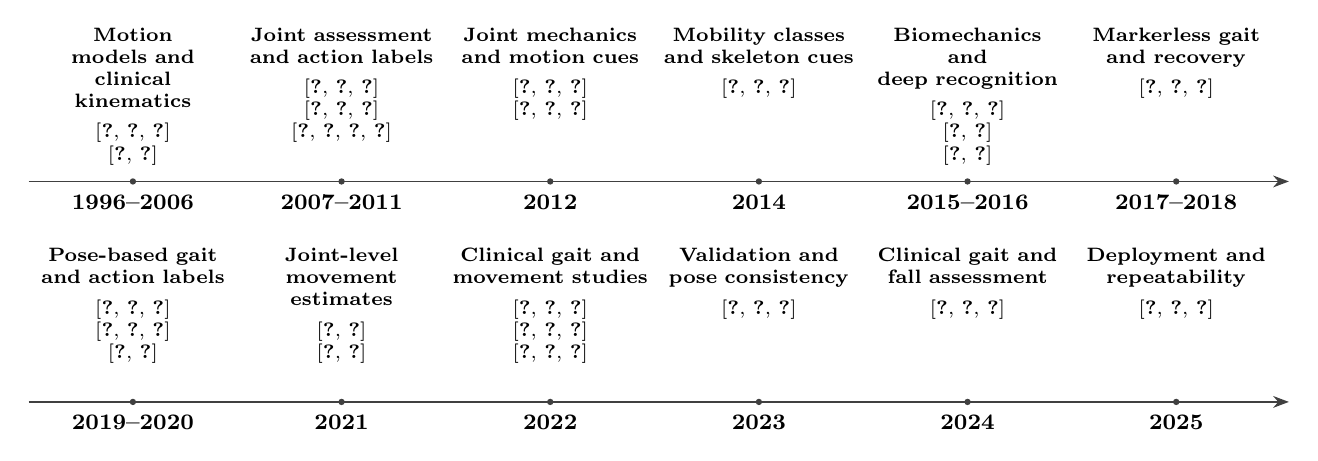
\begin{tikzpicture}[
  x=2.65cm, y=1cm,
  period/.style={anchor=north, font=\footnotesize\bfseries, inner sep=1pt},
  record/.style={anchor=north, text width=2.48cm, align=center, font=\scriptsize, inner sep=0pt},
  time axis/.style={-{Stealth[length=2mm]}, draw=black!75, line width=0.65pt}
]
\foreach \row in {0,-2.80} {
  \draw[time axis] (-0.50,\row) -- (5.54,\row);
  \foreach \slot in {0,1,2,3,4,5}
    \fill[black!75] (\slot,\row) circle[radius=1.15pt];
}
\foreach \years [count=\slot from 0] in {1996--2006,2007--2011,2012,2014,2015--2016,2017--2018}
  \node[period] at (\slot,-0.13) {\years};
\foreach \years [count=\slot from 0] in {2019--2020,2021,2022,2023,2024,2025}
  \node[period] at (\slot,-2.93) {\years};

\node[record] at (0,1.96) {\textbf{Motion models and\\clinical kinematics}\\[3pt]
  \cite{ju1996cardboard,kaufman2001gait,shakoor2003asymmetric}\\
  \cite{weidow2006hip,bejek2006influence}};
\node[record] at (1,1.96) {\textbf{Joint assessment\\and action labels}\\[3pt]
  \cite{astephen2008biomechanical,butler2009gait,valderrabano2007gait}\\
  \cite{reilly2009role,kiss2010effect,mcclelland2007gait}\\
  \cite{kiss2011effect,mont2007gait,li2010action,uddin2011human}};
\node[record] at (2,1.96) {\textbf{Joint mechanics\\and motion cues}\\[3pt]
  \cite{harding2012body,simonsen2012gait,reininga2012subjects}\\
  \cite{da2012biomechanical,eitzen2012sagittal,wang2012mining}};
\node[record] at (3,1.96) {\textbf{Mobility classes\\and skeleton cues}\\[3pt]
  \cite{elbaz2014novel,laroche2014classification,vemulapalli2014human}};
\node[record] at (4,1.96) {\textbf{Biomechanics and\\deep recognition}\\[3pt]
  \cite{favre2016gait,phinyomark2016gender,du2015hierarchical}\\
  \cite{leightley2016automated,meyer2015biomechanical}\\
  \cite{qingguang2015gait,schmitt2015effect}};
\node[record] at (5,1.96) {\textbf{Markerless gait\\and recovery}\\[3pt]
  \cite{bkaczkowicz2018gait,prakash2018vision,ong2017efficacy}};

\node[record] at (0,-0.84) {\textbf{Pose-based gait\\and action labels}\\[3pt]
  \cite{caetano2019skeleton,ahmad2019action,ro2019effects}\\
  \cite{li2020human,rohan2020human,fan2020gaitpart}\\
  \cite{juri2020characterization,viswakumar2019human}};
\node[record] at (1,-0.84) {\textbf{Joint-level\\movement estimates}\\[3pt]
  \cite{ismailidis2021kinematic,stenum2021two}\\
  \cite{boswell2021neural,vafadar2021novel}};
\node[record] at (2,-0.84) {\textbf{Clinical gait and\\movement studies}\\[3pt]
  \cite{bacon2022relation,lv2022analysis,uccheddu2022rgb}\\
  \cite{ma2022wushu,sharma2022surya,cotton2022transforming}\\
  \cite{armstrong2022novel,suhendar2022skeletal,yadav2022skeleton}};
\node[record] at (3,-0.84) {\textbf{Validation and\\pose consistency}\\[3pt]
  \cite{van2023accuracy,sheu2023improvement,marusic2023evaluating}};
\node[record] at (4,-0.84) {\textbf{Clinical gait and\\fall assessment}\\[3pt]
  \cite{blasco2024computer,stenum2024clinical,wang2024markerless}};
\node[record] at (5,-0.84) {\textbf{Deployment and\\repeatability}\\[3pt]
  \cite{doong2025predicting,yan2025efficient,schoenwether2025reliability}};
\end{tikzpicture}
\caption{Selected studies on joint mobility, gait analysis, human action recognition and pose estimation by publication period. The upper timeline runs from 1996 to 2018 and the lower timeline continues from 2019 to 2025.}
\label{fig:literature_timeline}
\end{figure}


\subsection{\rev{Fall-related gait recognition using vision and sEMG}}
\label{sec:fall_related}
\begin{revision}
The studies in Table~\ref{tab:fall_evidence} classify walking patterns associated with falls. Chen et al. \cite{chen2022computer} use camera-derived kinematics. Zhang et al. \cite{zhang2025myoelectric} compare classifiers using muscle activity, and Zhang et al. \cite{zhang2024fall} examine how much sEMG data a model needs to adapt to a new participant. Video and sEMG therefore describe different aspects of the same movement, namely its visible kinematics and the electrical activity of the muscles.

In all three studies the endpoint was recognition of gait patterns performed by healthy volunteers. The reported accuracies apply to the individual protocols. A comparison of the modalities would require a common cohort, task and evaluation. Using these outputs to assess a joint disorder would require clinically defined labels in patients, while a claim about future falls would require prospective follow-up.
\end{revision}

{\small\setlength{\tabcolsep}{4pt}\renewcommand{\arraystretch}{1.14}
\begin{table}[!htbp]
\centering\small
\caption{\rev{Fall-related gait-pattern recognition using video and surface electromyography. Accuracies refer to each study's own evaluation protocol.}}\label{tab:fall_evidence}
\begin{tabular}{>{\raggedright\arraybackslash}p{2.5cm}p{3.2cm}p{5.0cm}p{4.9cm}}
\toprule\rev{Study} & \rev{Signal and participants} & \rev{Reported task and finding} & \rev{Interpretive limit}\\\midrule
\rev{Chen et al. (2022) \cite{chen2022computer}} & \rev{Azure Kinect, seven healthy adults.} & \rev{Classified normal, pelvic-obliquity and knee-hyperextension gait with an 80/20 training and evaluation split. The support vector machine achieved $(94.9\pm3.36)\%$ accuracy.} & \rev{Illustrates visual pattern recognition in a controlled treadmill task. Clinical generalisation requires testing in patients.}\\\midrule
\rev{Zhang et al. (2025) \cite{zhang2025myoelectric}} & \rev{sEMG from eight lower-limb muscles in seven healthy participants.} & \rev{Compared classifiers for normal and abnormal gait patterns. A convolutional network with a bidirectional long short-term memory layer achieved $96.28\%$ accuracy.} & \rev{Shows that muscle signals carry information about the gait patterns under the tested protocol.}\\\midrule
\rev{Zhang et al. (2024) \cite{zhang2024fall}} & \rev{sEMG from eight lower-limb muscles in fifteen healthy participants.} & \rev{Compared eight adaptation schemes for recognising gait patterns in new participants. The hybrid model performed better than the tested baselines with limited target data.} & \rev{Shows how target-participant data can reduce the burden of adapting a model. The clinical value of such adaptation remains to be tested.}\\\bottomrule
\end{tabular}
\end{table}}

\FloatBarrier
\subsection{\rev{Evidence supporting joint-level interpretation}}
\label{sec:KO}
\begin{revision}
Figure~\ref{AnalysisJMP} shows where action recognition, pose estimation and gait analysis can contribute to joint assessment. A pose detector, an abnormal-gait classifier and a severity model may use the same underlying architecture while providing different outputs. Table~\ref{tab:validation_claims} links those outputs to the joint-level targets in Table~\ref{tab:joint_targets} and identifies the evidence needed for each use.

A video may show reduced knee flexion. Explaining that reduction requires information about the patient, including pain, walking speed and possible compensation at adjacent joints. A classifier trained to distinguish patient groups addresses a separate question and needs evaluation against clinical labels. The distinction matters when choosing a model and when reporting what its output can support.
\end{revision}

{\small\setlength{\tabcolsep}{4pt}\renewcommand{\arraystretch}{1.13}
\begin{table}[!htbp]
\centering\small
\caption{\rev{Validation needed for different uses of vision-based joint-mobility assessment.}}\label{tab:validation_claims}
\begin{tabular}{>{\raggedright\arraybackslash}p{3.0cm}p{5.8cm}p{6.8cm}}
\toprule\rev{Intended use} & \rev{Evidence needed} & \rev{Example of the validation question}\\\midrule
\rev{Movement measurement} & \rev{Matched anatomical definitions and reference measurements, errors by joint and gait phase, and repeatability.} & \rev{Do knee angles from video agree with motion capture during late stance and across repeat recordings?}\\\midrule
\rev{Gait-pattern recognition} & \rev{Defined labels, participant-separated evaluation, class-specific performance and uncertainty.} & \rev{Can the model recognise knee hyperextension in participants it has never seen?}\\\midrule
\rev{Joint disorder or severity} & \rev{Clinically defined targets, representative patients, assessment of confounders and independent validation.} & \rev{Does a camera-derived knee score distinguish clinically defined functional severity after accounting for walking speed?}\\\midrule
\rev{Longitudinal change} & \rev{Repeated measurements, measurement-error estimates and comparison with changes in clinical function.} & \rev{Does a change in post-treatment hip excursion exceed the error of repeat video measurements?}\\\midrule
\rev{Future-fall prediction} & \rev{A defined time horizon, prospectively observed falls, calibration and validation in the intended population.} & \rev{Does a predicted risk at a given time horizon correspond to the observed rate of falls?}\\\bottomrule
\end{tabular}
\end{table}}

\begin{figure}[t]
    \centering
    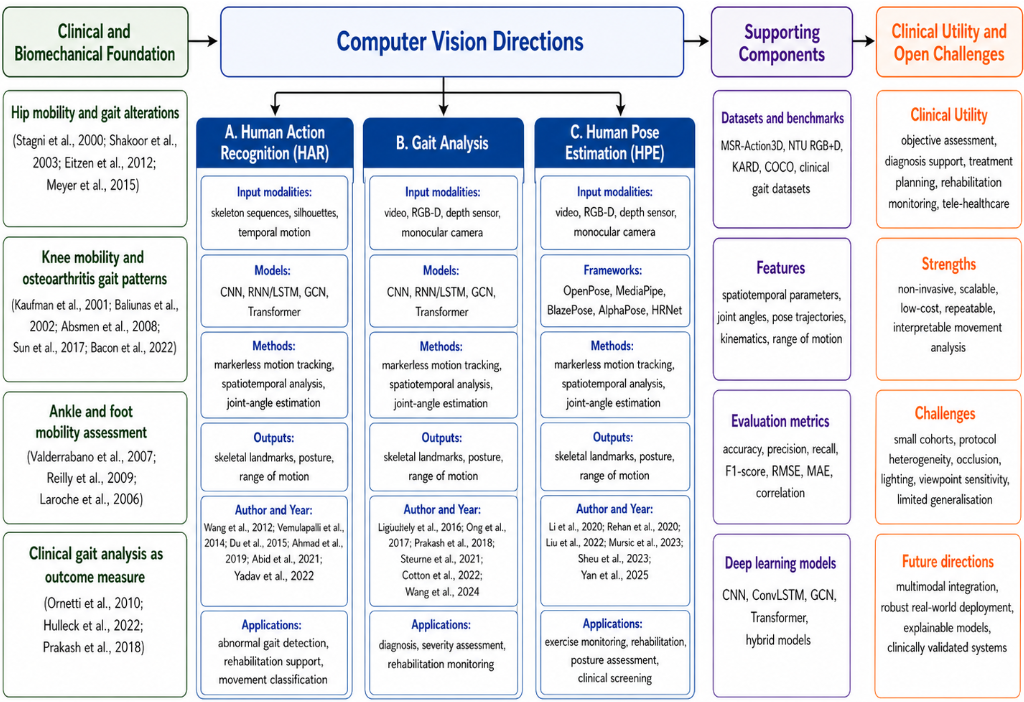
\includegraphics[width=400pt]{Images/Analysis_joint_mobility_diagram.pdf}
    \caption{An overview of computer vision directions for joint mobility assessment.}
    \label{AnalysisJMP}
\end{figure}

\FloatBarrier
\section{Discussion and Research Directions}
\label{sec:discussion}
\begin{revision}
The comparison by joint points to different priorities for hip, knee and ankle assessment. At the hip, both limbs and the trunk help reveal compensation. At the knee, walking speed and symptoms affect the interpretation of angle trajectories and loading estimates. At the ankle, foot landmarks and viewing geometry can determine whether an angle is measurable at all. Scataglini et al. \cite{scataglini2024accuracy} document differences in agreement across joints and gait variables. Tables~\ref{tab:joint_targets} and~\ref{tab:validation_claims} extend that measurement perspective to pattern recognition, severity assessment and monitoring change.
\end{revision}

\subsection{Discussion of the research questions}
\label{sec:rq_discussion}

\noindent\textbf{RQ1. How does joint impairment change gait?}
Hip studies identify changes in hip excursion and compensatory movement of the pelvis and trunk \cite{eitzen2012sagittal,reininga2012subjects}. Knee studies link changes in flexion, step regularity and loading to factors that include pain, speed and body mass \cite{kaufman2001gait,harding2012body,bacon2022relation}. Ankle studies draw attention to dorsiflexion, plantar flexion and propulsion, including residual differences after joint replacement \cite{valderrabano2007gait,schmitt2015effect}. These changes can extend to adjacent joints. The greater coverage of knee motion than ankle motion in Table~\ref{tableCV} also shows why the strength of the evidence varies by joint and plane.

\noindent\textbf{RQ2. What can vision methods recover from walking video?}
Pose estimation provides landmarks that can be tracked over a stride. Gait analysis uses them to estimate variables such as step timing and joint angles, and action recognition uses temporal patterns to assign movement labels \cite{stenum2021two,lv2022analysis,rohan2020human}. The intended output determines the choice of method. Detecting knee hyperextension as a pattern and measuring its peak angle call for different evaluations. Estimates of loading require a biomechanical or learned model whose output is checked against a suitable reference \cite{boswell2021neural}.

\Needspace{6\baselineskip}
\noindent\textbf{RQ3. What evidence supports measurement, severity and change?}
Agreement with a synchronised reference helps establish measurement accuracy when the anatomical definition, plane and gait phase match. A severity claim needs a clinically defined target and evaluation in patients who were held out during model development. Tracking recovery also requires repeatability and evidence that the observed change exceeds measurement error and relates to clinical function \cite{stenum2024clinical,schoenwether2025reliability}. Table~\ref{tab:validation_claims} sets out these requirements. The fall-related studies in Table~\ref{tab:fall_evidence} support recognition of scripted patterns, while a future-fall claim requires prospective outcomes.

\noindent\textbf{RQ4. When do recording conditions and the study population limit use?}
Camera placement and limb visibility affect the accuracy of joint angles. Occluding the far leg, for instance, can widen the limits of agreement during walking \cite{wade2023examination}. Clothing and lighting also affect landmark tracking, and validation across everyday conditions remains uneven (Section~\ref{sec:recording_robustness}). Results from healthy volunteers establish performance for the participants and conditions studied. Evaluating new patients, recording setups and sites helps determine where a method can be used and how often it produces a reportable measurement.


\subsection{\revred{Recording conditions that affect gait estimates}}
\label{sec:recording_robustness}
\begin{redrevision}
$-$\noindent\textbf{Limb self-occlusion during swing.}
In a side view, the leg farther from the camera can pass behind the nearer leg during swing. A pose estimator may miss the ankle or toe, or assign landmarks to the wrong leg. In their OpenPose workflow, Stenum et al. \cite{stenum2021two} inspected and corrected left--right switches and interpolated short gaps of up to 0.12\,s. Those corrections were part of the reported workflow, so its agreement with motion capture should be interpreted in light of that manual input. Wade et al. \cite{wade2023examination} found that sagittal hip and knee angle limits of agreement were about twice as wide on the occluded side as on the visible side during walking. Differences in foot and ankle landmark locations were also pronounced around push-off and swing. A whole-cycle average can therefore hide errors in the part of the stride used to assess foot clearance or peak flexion.

Temporal tracking can help maintain left--right identity and bridge brief gaps using frames in which the joint is visible. A second view can add information when one leg hides the other. OpenCap, for example, weights landmarks by their confidence when combining synchronised views to estimate three-dimensional positions \cite{uhlrich2023opencap}. It then uses a sequence model to estimate additional landmarks. A sustained loss of visibility still leaves the trajectory dependent on the model's assumptions. For outcomes such as peak knee flexion, studies should report when a peak falls inside an interpolated interval and how often the affected cycle has to be excluded.

$-$\noindent\textbf{Loose clothing.}
Draped fabric can hide a knee or ankle contour and move differently from the limb underneath. Frame-by-frame pose models infer the joint from the visible parts of the body and the relationship between them. Multi-camera systems can also combine cues across views and fit an articulated body model. Augustine et al. \cite{augustine2025clothing} reported root mean square differences below \(2^\circ\) between tight and loose clothing conditions with an eight-camera Theia3D setup in healthy adults. This was a comparison of estimates across clothing conditions. Agreement with an independent anatomical reference would require a separate test.

Viswakumar et al. \cite{viswakumar2022omgait} obtained joint-angle curves from smartphone videos of volunteers wearing garments such as sarees and dhotis. Their benchmark was a normative gait database. The study supports feasibility for those garments, while the agreement of a patient's angles with a simultaneous reference remains a separate question. Clothing variation in training and checks for unstable landmark tracks are plausible ways to improve performance. Their benefit should be tested on garments and participants that the model has not seen, with errors reported separately by joint.

$-$\noindent\textbf{Changing light and background.}
Moving shadows, backlighting and exposure changes can reduce the contrast around a foot or knee over part of a stride. Movement behind the person can also make it harder to keep the same person in view. Viswakumar et al. \cite{viswakumar2022omgait} tested fixed lighting levels, from approximately 50 to 9{,}800\,lux, in separate walking conditions. Their results characterise those lighting conditions. A walking trial in which illumination changes mid-stride tests a different source of error.

Models can address poor illumination at training time. Lee et al. \cite{lee2023lowlight}, for instance, used aligned low-light and well-lit images to train a pose estimator for dark images. Wu et al. \cite{wu2012illumination} estimated illumination and body pose together across frames in a multi-camera system. These studies evaluate pose estimation or full-body tracking. To establish whether these approaches improve clinical gait measurement, studies would need to compare their joint-angle estimates with a synchronised reference during the lighting transition. A practical video pipeline can also track the same person throughout the clip and flag frames with severe blur, clipping or missing landmarks for review.

$-$\noindent\textbf{How to test robustness.}
Assessments should include repeated walks under controlled changes in visibility, clothing and light, with the same outcome measured against a synchronised reference. Useful reports give error and agreement by joint, side and gait phase, as well as the share of frames and cycles that were corrected, interpolated or rejected. A method that reports accurate angles only for successful recordings may still miss the patients or gait phases of greatest clinical interest.
\end{redrevision}

\subsection{\rev{Generalisation and clinical interpretation}}
\begin{revision}
Participant separation is essential when evaluating a model intended for a new patient. Windows or gait cycles from the same person can share appearance, anatomy and recording conditions. A test set containing related observations therefore answers a different question from a test involving unseen participants or a separate clinic. Studies should state the splitting unit and distinguish within-participant, cross-participant and external validation. When adaptation uses data from a new participant, its amount and role must be reported separately from the final test data.

Clinical interpretation also depends on variables that video may not reveal. Pain, walking speed, body mass, prior treatment and compensation can affect the same gait feature \cite{bejek2006influence,harding2012body,ro2019effects,bacon2022relation}. A model may learn one of these correlates rather than the intended disorder. Evaluations should therefore describe relevant patient characteristics, test appropriate subgroup performance and avoid interpreting a group difference as a causal explanation. Estimates of joint moments require particular care because they depend on learned or biomechanical assumptions beyond the visible trajectory \cite{boswell2021neural}.

The sEMG studies in Section~\ref{sec:fall_related} suggest useful complementary information about muscle activation, but the benefit of combining it with video remains a question for evaluation. Any proposed fusion system should compare video alone, sEMG alone and their combination on the same participants and outcome. Additional sensing should be justified by a measurable benefit relative to acquisition burden, rather than assumed to improve assessment.

\noindent\textbf{Limits of this synthesis.} The studies use different instruments, participant groups and outcome definitions. The narrative comparison identifies patterns in the evidence and open validation questions. Estimating a pooled effect or ranking methods would require comparable measurement protocols and clinical outcomes. Studies involving healthy volunteers and other movement tasks inform the choice of methods. Studies in patients are needed to estimate the benefit of those methods in routine care.
\end{revision}

\Needspace{10\baselineskip}
\subsection{\rev{Research directions}}
\label{sec:research_directions}
\begin{revision}
Future studies should establish which video measures can be used reliably in clinics, rehabilitation and home monitoring. The required evidence depends on the outcome and the decision it is intended to support.

\begin{itemize}
    \item \textbf{Clinically representative datasets.}
    Recruit participants across hip, knee and ankle conditions, severity levels, ages and body types. Record symptoms, walking speed, treatment history and compensation alongside synchronised reference measurements \cite{kaufman2001gait,weidow2006hip,ro2019effects,bacon2022relation}. Hold out participants and, where possible, clinical sites when assessing generalisation.

    \item \textbf{Biomechanical interpretability.}
    Connect a model's output to observable quantities such as joint-angle trajectories, asymmetry, range of motion or stance and swing timing \cite{ornetti2010gait,andriacchi2006role,astephen2008biomechanical,favre2016gait}. Specify the motion plane and gait phase and report how changes in walking speed or compensation affect the interpretation. Validate loading estimates against an appropriate biomechanical reference.

    \item \textbf{Multimodal assessment.}
    Pair video with inertial signals, muscle activity or clinical measures when they can add information about the outcome \cite{juri2020characterization,zhang2025myoelectric,zhang2024fall}. Compare the individual inputs and their combination on the same participants and task. That comparison can show whether any gain justifies the additional equipment and recording effort.

    \item \textbf{Robustness in everyday settings.}
    Record the same walks across relevant viewpoints, clothing, illumination and occlusion conditions \cite{ong2017efficacy,viswakumar2022omgait,van2023accuracy,wade2023examination}. Report error by joint and gait phase as well as the proportion of recordings that require correction or repetition. These measures are especially important when a method is intended for unsupervised home use.

    \item \textbf{Longitudinal and outcome-oriented validation.}
    Use repeat recordings to quantify measurement error and test whether video can detect functional changes during rehabilitation or disease progression \cite{gaudreault2011effects,bkaczkowicz2018gait,stenum2024clinical}. Relate observed changes to an appropriate clinical measure and evaluate whether they inform follow-up decisions.

    \item \textbf{Lightweight models for routine use.}
    Test portable systems on the devices and in the settings for which they are intended \cite{li2020human,uccheddu2022rgb,yan2025efficient}. Alongside runtime and acquisition effort, report agreement for the target joint variables. Efficient landmark estimation is most useful when the resulting gait measures retain their accuracy.

    \item \textbf{Clinical integration.}
    Work with clinicians and patients to decide which measurements fit a musculoskeletal assessment and how uncertainty should be reported. Pain, prior treatment and comorbidities can affect the interpretation of the same movement pattern \cite{hertling2006management,lu2026musculoskeletal,pandey2022movement}. Workflow evaluations should examine whether the output supports a decision and how much effort it takes to obtain.
\end{itemize}

These directions connect technical development to the practical question of when a gait measure is reliable enough to guide assessment. They also provide a basis for comparing systems tested in different settings.
\end{revision}


\Needspace{17\baselineskip}
\section{Conclusion}
\label{sec:conclusion}
\begin{revision}
This survey reviewed clinical and computer vision approaches to identifying and assessing mobility problems at the hip, knee and ankle. Clinical studies show that impairment changes movement at the affected joint and can alter coordination elsewhere in the lower limb. Instrumented gait analysis has helped characterise these changes through measures of timing, joint motion and loading, often alongside measures of pain and function. Advances in pose estimation, gait analysis and human action recognition now make it possible to estimate selected movement variables from RGB and RGB-D video with less specialised equipment. The reviewed studies range from general movement recognition to more clinically focused work on abnormal gait and rehabilitation. What each study establishes depends on its outcome and reference. An angle estimate needs agreement with a matched measurement, a severity assessment needs clinically defined labels, and tracking recovery requires a repeatable measure that captures meaningful change. The fall-related studies illustrate recognition of gait patterns performed by healthy volunteers, and prospective data would be needed to predict future falls. Small cohorts, inconsistent protocols and sensitivity to camera placement, visibility, clothing and lighting still limit clinical use. Representative patient data and testing in realistic settings will help determine which measures can support repeated assessment. Joint-specific validation and collaboration with clinicians will be important if video-based gait analysis is to inform routine care and rehabilitation.
\end{revision}
\begingroup\small
\bibliographystyle{unsrtnat}
\bibliography{bibliography}
\endgroup

\end{document}
